%==============================================================================
% PhD defense deck -- Solal Rapaport
% The Impact of Repository Mutability for Software Integrity and Supply-Chain Security.
% Self-contained: theme (beamerthemetptng.sty) and logo PDFs live in defense/;
% figures are resolved from the two conference talks via \graphicspath below,
% and every numeric macro is embedded directly in this file.
%
% Build from defense/ :  latexmk -pdf slides.tex   (or pdflatex twice)
%==============================================================================
\documentclass[aspectratio=169]{beamer}
\usepackage[utf8]{inputenc}

\mode<presentation>
% Institutional theme ships as a local .sty next to this file.
\IfFileExists{beamerthemetptng.sty}{%
  \usetheme{tptng}%
  \iftptusefontspec
    \setmonofont{inconsolata}%
  \else
    \usepackage[T1]{fontenc}%
    \usepackage{inconsolata}%
  \fi
}{%
  \usetheme{Madrid}%
  \usepackage[T1]{fontenc}%
  \usepackage{inconsolata}%
}

% Resolve every figure from the two talks WITHOUT copying them locally.
\graphicspath{%
  {pdfs/}%
  {previous_talks/REP_talk/figs/}{previous_talks/REP_talk/pdfs/}%
  {previous_talks/ASE_talk/figs/}{previous_talks/ASE_talk/pdfs/}%
  {previous_talks/SWHSec/figs/}{previous_talks/SWHSec/pdfs/}%
  {../chapters/chapter02/fig02/}{../figures/}%
}
\DeclareGraphicsExtensions{.pdf,.png,.jpg,.jpeg}
\usepackage{figlatex}

\usepackage[english]{babel}
\usepackage[babel]{microtype}
\usepackage{booktabs}
\usepackage{tikz}
\usetikzlibrary{positioning}
\usepackage{calc}
\usepackage[useregional]{datetime2}
\usepackage{multirow}
\usepackage{amsmath,amssymb,amsfonts}
\usepackage{graphicx}
\usepackage{siunitx}
\sisetup{detect-all=true}
\usepackage{textcomp}
\usepackage{xcolor}
\usepackage{xspace}
\usepackage[normalem]{ulem}
\usepackage{verbatim}
\usepackage{url}
\usepackage{makecell}
\usepackage{listings}
\usepackage[most]{tcolorbox}
\tcbuselibrary{listings}

% Numeric inline citations ([3,7-9] compressed) resolved by the References frames.
\usepackage[numbers,sort&compress]{natbib}
\setbeamertemplate{bibliography item}[text]   % numbered markers, not beamer icons

\lstdefinelanguage{bash}{morekeywords={git,cd},sensitive=true}
\lstset{basicstyle=\ttfamily\footnotesize,breaklines=true,frame=single,columns=fullflexible}
\lstdefinestyle{bashtiny}{basicstyle=\ttfamily\tiny,breaklines=true,frame=single,columns=fullflexible}

\newtcblisting{terminalbox}{
    listing only,
    colback=black,
    coltext=green!70!white,
    fontupper=\ttfamily\small\bfseries,
    arc=3mm,
    boxrule=0pt,
    left=8pt,
    right=8pt,
    top=3pt,
    bottom=3pt,
    breakable,
    listing options={
        basicstyle=\ttfamily\small\bfseries\color{green!70!white},
        frame=none,
        breaklines=true
    }
}
\newtcblisting{terminalboxsmall}{
    listing only,
    colback=black,
    coltext=green!70!white,
    fontupper=\ttfamily\footnotesize\bfseries,
    arc=3mm,
    boxrule=0pt,
    left=6pt,
    right=6pt,
    top=2pt,
    bottom=2pt,
    breakable,
    listing options={
        basicstyle=\ttfamily\footnotesize\bfseries\color{green!70!white},
        frame=none,
        breaklines=true
    }
}

% Side text+figure layouts: pull into the theme left margin (24mm frieze)
% so text sits further left and the figure can grow.
\newcommand{\sidefigbegin}{%
  \hspace*{-14mm}%
  \begin{minipage}{\dimexpr\textwidth+14mm\relax}%
  \setlength{\leftmargini}{0.9em}%
}
\newcommand{\sidefigend}{\end{minipage}}

%==============================================================================
% Embedded numeric macros (merged from REP_talk/numbers.tex,
% ASE hardcoded numbers, and Chapter 5 counts). Everything in slides.tex.
%==============================================================================
% --- Study 1: tags (from REP_talk/numbers.tex) ---
\newcommand{\CutoffDate}{February 23, 2016\xspace}
\newcommand{\TemporalSpan}{2017--2025\xspace}
\newcommand{\OriginsWithTagsShort}{\num{45.5}\,M\xspace}
\newcommand{\TotalTagsShort}{\num{3.2}\,B\xspace}
\newcommand{\TotalAlterationsShort}{\num{10.2}\,M\xspace}
\newcommand{\AlteredRepositoriesShort}{\num{189}\,k\xspace}
\newcommand{\AlteredRepositoriesPercent}{\num{0.41}\%\xspace}
\newcommand{\LegitMovesShort}{\num{626}\,k\xspace}
\newcommand{\DeletionsShort}{\num{9.5}\,M\xspace}
\newcommand{\DeletionsPercent}{\num{93.85}\%\xspace}
\newcommand{\LegitMovesPercentOfAlterations}{\num{6.15}\%\xspace}
\newcommand{\MovesWithContentChangeShort}{\num{427}\,k\xspace}
\newcommand{\PercentMovesContentChange}{\num{68.15}\%\xspace}
\newcommand{\NixPkgsTracked}{\num{2407}\xspace}
\newcommand{\NixPkgsAffected}{\num{32}\xspace}
\newcommand{\NixPkgsHashMismatch}{\num{7}\xspace}
\newcommand{\NixPkgsFailDeletion}{\num{4}\xspace}
\newcommand{\NixPkgsFailHashMismatch}{\num{3}\xspace}
\newcommand{\AttackRepoFork}{\texttt{zendesk/changed-files}\xspace}
\newcommand{\AttackTagMovesCount}{\num{346}\xspace}
\newcommand{\AttackStableDaysLowerBound}{\num{148}\xspace}
\newcommand{\AttackStableCases}{\num{340}\xspace}
\newcommand{\StarPropZeroOnePct}{0.0248\%\xspace}
\newcommand{\StarPropZeroOnePctTrunc}{\num{0.02}\%\xspace}
\newcommand{\StarPropFiveHundredPlusPct}{0.7488\%\xspace}
\newcommand{\StarPropFiveHundredPlusPctTrunc}{\num{0.75}\%\xspace}
\newcommand{\StarZeroOneAlterationsPercent}{\num{74.29}\%\xspace}

% --- Study 2: histories (from ASE_talk/numbers.tex) ---
\newcommand{\FullDataset}{2024-08-23\xspace}
\newcommand{\SWHOriginShort}{\num{310}\,M\xspace}
\newcommand{\SWHRevisionsShort}{\num{4.2}\,B\xspace}
\newcommand{\OriginsTwoVisitsOrMoreShort}{\num{111}\,M\xspace}
\newcommand{\PercentOriginsAltered}{\num{1.10}\%\xspace}
\newcommand{\GitRootCauseCommitsShort}{\num{8.7}\,M\xspace}
\newcommand{\GitOriginsRootCauseCommitsShort}{\num{1.22}\,M\xspace}
\newcommand{\PercentMETARootCauseCommits}{\num{13.3}\%\xspace}
\newcommand{\PercentDIRRootCauseCommits}{\num{76.8}\%\xspace}
\newcommand{\PercentCategFileModified}{\num{62.7}\%\xspace}
\newcommand{\PercentCategFileRemoved}{\num{14.8}\%\xspace}
\newcommand{\PercentCategContentSplit}{\num{8.8}\%\xspace}
\newcommand{\PercentCategCommitterDate}{\num{9.9}\%\xspace}
\newcommand{\StarAlterRateZeroOne}{\num{0.3}\%\xspace}
\newcommand{\StarAlterRateThousandPlus}{\num{3.3}\%\xspace}
\newcommand{\LicenseAllShort}{\num{797}\,k\xspace}
\newcommand{\LicenseOriginsThousandPlus}{\num{76}\xspace}
\newcommand{\LicenseUpdate}{\num{79}\%\xspace}
\newcommand{\LicenseFullChange}{\num{14}\%\xspace}
\newcommand{\LicensePartialChange}{\num{5}\%\xspace}
\newcommand{\LicenseOrigins}{\num{32}\,k\xspace}
\newcommand{\SecretsRemovedAllShort}{\num{13}\,M\xspace}
\newcommand{\SecretsOriginsAllShort}{\num{75}\,k\xspace}

% --- Study 3: secrets (from Chapter 5) ---
\newcommand{\SecretFirstExtractionShort}{\num{365.6}\,M\xspace}
\newcommand{\SecretSecondExtractionShort}{\num{2.85}\,M\xspace}
\newcommand{\SecretResolvedBlobs}{\num{281728}\xspace}
\newcommand{\SecretFindingBlobs}{\num{25859}\xspace}
\newcommand{\SecretDetectionRate}{\SI{9.18}{\percent}\xspace}
\newcommand{\SecretPKValidBlobs}{\num{10038}\xspace}
\newcommand{\SecretPKFlaggedBlobs}{\num{11613}\xspace}
\newcommand{\SecretPKValidPct}{\SI{86.4}{\percent}\xspace}

% Section divider: re-show the outline with the current section highlighted,
% so the talk can be tracked against the opening roadmap.
\AtBeginSection[]{%
  \begin{frame}{Outline}
    \tableofcontents[currentsection]
  \end{frame}%
}
\AtBeginSubsection{}

%==============================================================================
% Title metadata (from models/LaTeX/1ere.tex; date still a placeholder).
%==============================================================================
% Title runs to four lines at the theme's 17pt; 14pt keeps it inside the
% fixed-height title minipage, clear of the author block below.
\setbeamerfont{title}{size*={14}{17},series=\bfseries}
\title[Repository Mutability]{The Impact of Repository Mutability\\ for Software Integrity\\ and Supply-Chain Security}
\subtitle{}
\author{Solal Rapaport}
\institute{\texttt{phd2026@solalr.com}}
\date[Defense --- October 2 2026]{PhD Defense --- October 2 2026}

\begin{document}

\maketitle

\begin{frame}{Doctoral committee}

    {\small
    \begin{tabular}{@{}lll@{}}
        \toprule
        \textbf{Name} & \textbf{Affiliation} & \textbf{Role} \\
        \midrule
        Samia Bouzefrane     & Professeure, CNAM                      & Reviewer \\
        Yvon Kermarrec       & Professeur, IMT-Atlantic               & Reviewer \\
        Christelle Urtado    & Professeure, IMT-Mines d'Ales          & Examiner \\
        Olivier Zendra       & Charg\'e de Recherche, INRIA           & Examiner \\
        Laurent Pautet       & Professeur, T\'el\'ecom Paris          & Supervisor \\
        Stefano Zacchiroli   & Professeur, T\'el\'ecom Paris          & Co-supervisor \\
        Samuel Tardieu       & Ma\^itre de Conf.,\ T\'el\'ecom Paris  & Co-supervisor \\
        Gregory Blanc        & Ma\^itre de Conf.,\ T\'el\'ecom SudParis & Guest \\
        \bottomrule
    \end{tabular}
    }

    \vspace{1em}

    {\small Thesis prepared at T\'el\'ecom Paris, Institut Polytechnique de Paris.}
\end{frame}

\begin{frame}{Outline}
    \tableofcontents
\end{frame}

%##############################################################################
\section{Supply Chain and Git}
%##############################################################################

% ------------------------------------------------------------------
\begin{frame}{Modern software is assembled, not written}
    \sidefigbegin
    \begin{columns}[T,totalwidth=\linewidth]
        \begin{column}{0.44\linewidth}
            {\small
            \begin{itemize}
                \item A deployable artifact can depend on \textbf{hundreds to thousands} of upstream components.
                \item Most ship as a \textbf{package}, picked by a \textbf{version label} (\texttt{2.3.1}) and fetched by a package manager: npm, PyPI, crates.io, Maven.
                \item \textbf{CI} installs and runs them on every change; \textbf{lockfiles}, \textbf{SBOMs}, SLSA provenance record what went in~\cite{ladisa2023supplychain,tamanna2024analyzingchallengesdeploymentslsa}.
                \item Premise: \emph{Resolving a dependency today yields the same artifact as yesterday.}
            \end{itemize}
            }
        \end{column}
        \begin{column}{0.54\linewidth}
            \begin{center}
                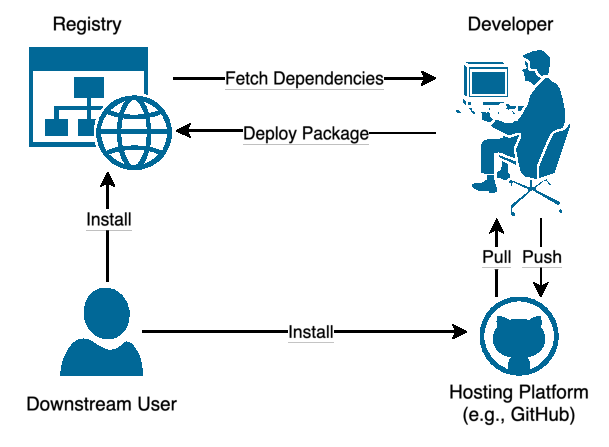
\includegraphics[width=\linewidth]{supply_chain.drawio.pdf}
            \end{center}
        \end{column}
    \end{columns}
    \sidefigend
\end{frame}

% ------------------------------------------------------------------
\begin{frame}{A public repository plays two roles at once}
    % \begingroup, not a brace group: a brace group here would be swallowed
    % as the frame subtitle.
    \begingroup\small
    \begin{itemize}\setlength{\itemsep}{0.4em}
        \item \textbf{Collaboration workspace:} developers push, pull, and reorganise work in progress. Rewriting recent work here is \textbf{accepted practice}.
        \item \textbf{Distribution point:} package managers, CI, auditors, and researchers consume the \emph{same} repository as an \textbf{external artifact}, where stability is expected.
        \item Downstream actors treat published \textbf{names / tags} as durable identifiers --- the repository becomes a \textbf{trust anchor}.
        \item \textbf{Thesis scope:} the mutability of the names and states a repository publishes --- not the full supply-chain attack surface.
    \end{itemize}
    \endgroup
    % \vspace{0.5em}
    % {\small\emph{One artefact, two incompatible sets of expectations.}}
\end{frame}

% --- CUT: merged into ``two roles'' above; Ladisa definition spoken ---
\iffalse
\begin{frame}{A public repository plays two roles at once}
    % \begingroup, not a brace group: a brace group here would be swallowed
    % as the frame subtitle.
    \begingroup\small
    \begin{itemize}\setlength{\itemsep}{0.3em}
        \item \textbf{Collaboration workspace:} developers push, pull, and reorganise work in progress. Rewriting recent work here is \textbf{accepted practice}.
        \item \textbf{Distribution point:} package managers, CI, auditors, and researchers consume the \emph{same} repository as an \textbf{external artifact}, where stability is expected.
        \item It publishes far more than files: commit metadata, branch and tag names, release objects.
        \item Downstream actors never see the change directly, so they treat published \textbf{names / tags} as durable identifiers --- the repository becomes a \textbf{trust anchor}.
    \end{itemize}
    \endgroup
    \vspace{0.3em}
    {\small\emph{One artefact, two incompatible sets of expectations.}}
\end{frame}

\begin{frame}{Supply-chain attacks and the repository attack surface}
    \begin{block}{Definition}
        \small A \textbf{software supply-chain attack} compromises downstream users \emph{not}
        by exploiting a flaw in their own code, but by manipulating an \textbf{upstream
        component} they depend on --- so victims execute attacker-controlled code through
        their normal build or update process~\cite{ladisa2023supplychain}.
    \end{block}
    \begin{itemize}
        \item \textbf{Technical surface:} version control, build systems, registries and
              distribution platforms, maintainer workstations~\cite{paloalto_unit42_2025}.
        \item \textbf{Social surface:} contributors, maintainers, administrators --- account
              compromise, social engineering, malicious contributions disguised as bug
              fixes~\cite{ladisa2023supplychain}.
        \item \textbf{Thesis scope:} the \textbf{mutability of the names and
              states a\\repository publishes}
    \end{itemize}
\end{frame}
\fi
% --- END CUT ---

% ------------------------------------------------------------------
% --- CUT: talk the object model over Git_arch ---
\iffalse
\begin{frame}{The Git object model: identity comes from content}
    \begin{itemize}
        \item \textbf{Blobs}, \textbf{trees}, \textbf{commits}, \textbf{releases} (annotated
              tags) --- each named by a \textbf{hash of its own content}: the identifier
              \emph{is} a fingerprint~\cite{ProGit2014}.
        \item A commit's hash covers its parents too $\Rightarrow$ a \textbf{Merkle DAG}: one
              known commit ID verifies everything reachable from it (SHA-1 collisions
              notwithstanding~\cite{stevens2017shattered}).
        \item Note what sits \emph{outside} the DAG: \textbf{branches and tags}, attached at
              the repository boundary.
    \end{itemize}
\end{frame}
\fi
% --- END CUT ---

% ------------------------------------------------------------------
\begin{frame}{Objects inside the DAG, references at the boundary}
    \hspace*{-14mm}%
    \begin{minipage}{\dimexpr\textwidth+14mm\relax}
    \centering
    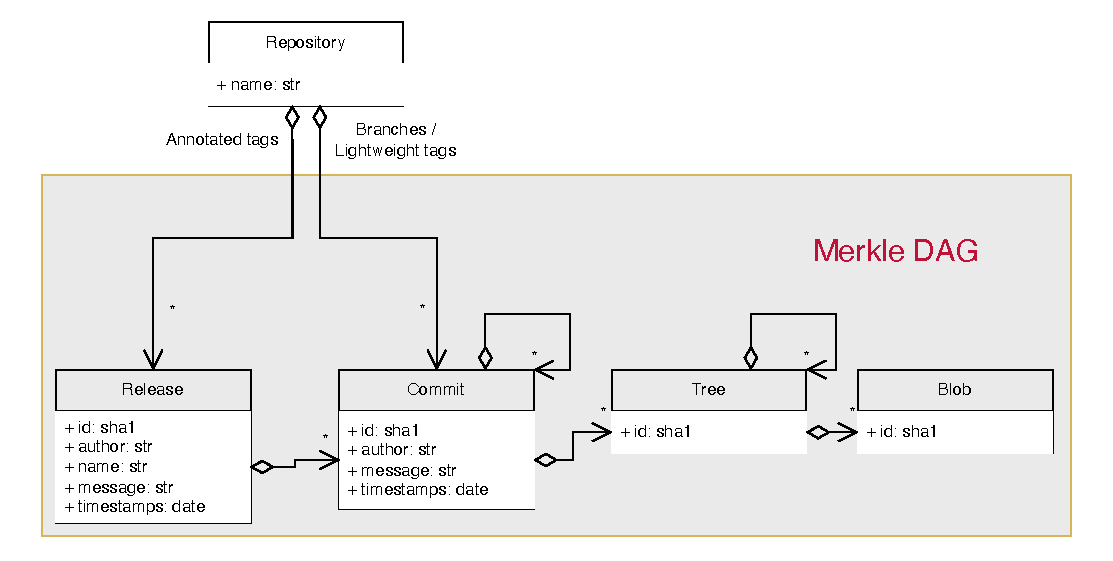
\includegraphics[width=\linewidth,height=0.78\textheight,keepaspectratio]{Git_arch.drawio.pdf}\\[0.3em]
    {\small Hashes name objects \emph{inside} the DAG; \textbf{branches and tags} sit at the boundary.}
    \end{minipage}
\end{frame}

% --- CUT: talk branch-vs-tag and force-push over git_amend ---
\iffalse
\begin{frame}{References: mutable names on top of immutable objects}
    \begin{itemize}
        \item Users do not always handle hashes. They handle \textbf{references}:
              branches (\texttt{refs/heads/}) and tags (\texttt{refs/tags/})~\cite{ProGit2014}.
        \item \textbf{Branches are meant to move.} \texttt{main} points at the newest commit
              of a development line; advancing it is ordinary and visible.
        \item \textbf{Tags carry a different social role:} they mark releases, and release
              workflows treat the name as a stable identifier.
        \item Yet Git lets \textbf{any} tag ref be deleted or retargeted. Annotated tags add a
              metadata object --- \textbf{not} immutability~\cite{git_tag_retagging_docs}.
        \item \textbf{Why?} Distributed design: two clones may bind the same tag name to
              different commits, and the protocol cannot preserve both. Flexibility was chosen
              over protocol-level immutability of release labels~\cite{torvalds_retagging_2007}.
    \end{itemize}
\end{frame}

\begin{frame}{How published history actually changes}
    \begin{itemize}
        \item \texttt{git commit --amend} replaces a recent commit;
              \texttt{git rebase} replays, reorders, squashes, or splits a
              range~\cite{ProGit2014}.
        \item Nothing mutates in place: Git writes \textbf{new} objects, and the old ones merely
              become \textbf{unreachable} from the public refs.
        \item A commit ID covers its parents, so one edit forces \textbf{every descendant} to be
              replaced --- the \textbf{snowball effect}. Then \texttt{push --force} moves the
              public ref to a commit that does not extend the previous history.
    \end{itemize}
\end{frame}
\fi
% --- END CUT ---

% ------------------------------------------------------------------
\begin{frame}{Amend and rebase: new objects, orphaned originals}
    \hspace*{-14mm}%
    \begin{minipage}{\dimexpr\textwidth+14mm\relax}
    \centering
    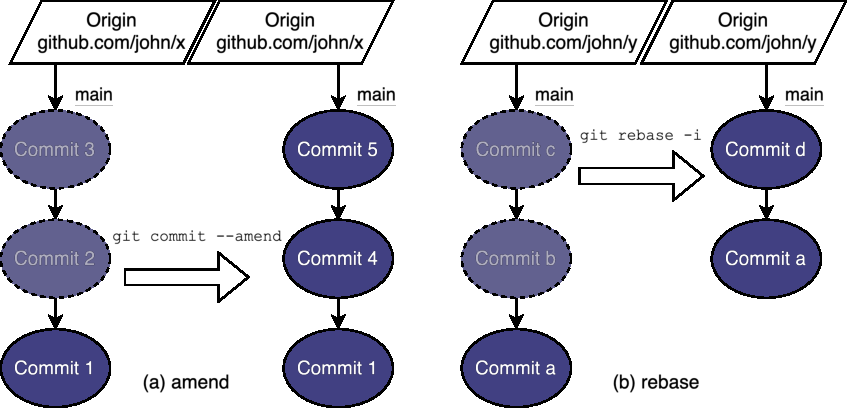
\includegraphics[width=\linewidth,height=0.76\textheight,keepaspectratio]{git_amend.drawio.pdf}\\[0.25em]
    {\small Branches are meant to move; \textbf{tags} are treated as stable \\ yet any ref can be deleted or retargeted, then \texttt{push --force}.}
    \end{minipage}
\end{frame}

% ------------------------------------------------------------------
\begin{frame}{Three properties at stake}
    \begin{itemize}
        \item \textbf{Safety} --- protection against \emph{non-adversarial} failure: accidental
              loss, a previously published state becoming unavailable, builds whose inputs
              silently change.
        \item \textbf{Reproducibility} --- a recorded build input still identifies the same
              source artifact later; the basis of auditing and reproducible
              builds~\cite{DBLP:journals/software/LambZ22}.
        \item \textbf{Security} --- protection against \emph{deliberate} manipulation:
              \emph{integrity} (a reference keeps designating the state a consumer verified)
              and \emph{confidentiality} (credentials do not leak through the published tree).
    \end{itemize}
    \vspace{0.5em}
    {\small The \emph{same} operation can be a benign release correction or an attack, and
     intent is not observable from archival evidence. This thesis therefore measures
     \textbf{observable effects}, not motives.}
\end{frame}

%##############################################################################
\section{Motivation}
%##############################################################################

% ------------------------------------------------------------------
\begin{frame}[fragile]{March 2025: a tag that changed meaning}
    \begin{itemize}
        \item \texttt{tj-actions/changed-files}: a widely reused GitHub Actions helper.
        \item Attackers retargeted \AttackTagMovesCount{} existing versions
              (\texttt{v39}\dots\texttt{v47}) to \textbf{one malicious
              commit}~\cite{paloalto_unit42_2025}.
        \item \AttackStableCases{} of those tags had been stable
              $\geq\AttackStableDaysLowerBound{}$ days --- trusted pins, not fresh noise.
        \item Anyone resolving a familiar version name then \textbf{ran attacker code}
              that could leak developer credentials.
    \end{itemize}
    \vspace{0.3em}
    \begin{terminalbox}
$ # your workflow, unchanged:
$ uses: tj-actions/changed-files@v45
$ # same name -> different code after the next fetch
    \end{terminalbox}
    \vspace{0.2em}
    {\small No downstream vulnerability was needed --- only an ordinary reference update.}
\end{frame}

% ------------------------------------------------------------------
% ------------------------------------------------------------------
\begin{frame}{Thesis question and three nested layers}
    \begin{block}{Central question}
        {\small Can changes that undermine trust in a repository be \textbf{detected after the fact},
        \textbf{at ecosystem scale}, and \textbf{classified}?}
    \end{block}
    \vspace{0.05em}
    \begin{center}
    \begin{tikzpicture}[
        layer/.style={draw=tptred, line width=0.8pt, rounded corners=2pt,
                      text width=0.90\linewidth, inner xsep=6pt, inner ysep=2.5pt, align=left}
    ]
        \node[layer] (l1) {\footnotesize\textbf{Layer 1 --- Tags}\quad
            A release \emph{name} can resolve to different code while it persists in workflows.};
        \node[layer, below=3pt of l1] (l2) {\footnotesize\textbf{Layer 2 --- History}\quad
            A published \emph{commit graph} can be replaced: the branch seems to advance, the past is rewritten.};
        \node[layer, below=3pt of l2] (l3) {\footnotesize\textbf{Layer 3 --- Content}\quad
            A \emph{file removed} during a rewrite may survive in clones and archives --- possibly secrets.};
    \end{tikzpicture}
    \end{center}
    % \vspace{0.25em}
    % {\footnotesize Study~1 / Ch.\,3 \quad$\cdot$\quad Study~2 / Ch.\,4 \quad$\cdot$\quad Study~3 / Ch.\,5.
    %  One method: compare archival snapshots, then filter and classify.}
\end{frame}

% --- CUT: merged into ``thesis question and three nested layers'' ---
\iffalse
\begin{frame}{One problem at three nested layers}
    \begin{itemize}
        \item \textbf{Layer 1 --- Reference:} a release \emph{tag} can resolve to different
              code over time while its name persists in registries and workflows.
        \item \textbf{Layer 2 --- History:} a published \emph{commit history} can be
              replaced, so a branch that seems to advance instead rewrites its past.
        \item \textbf{Layer 3 --- Content:} a \emph{file removed} during such a rewrite may
              survive in clones and archives --- possibly containing secrets.
    \end{itemize}
    \vspace{0.6em}
    {\small Each layer goes deeper into repository state; each needs its own detection and
     classification, and none should be labelled an ``attack'' by default.}
\end{frame}

\begin{frame}{Thesis question and three studies}
    \begin{block}{Central question}
        Can changes that undermine trust in a repository be \textbf{detected after the fact},
        \textbf{at ecosystem scale}, and \textbf{classified} without treating every
        maintenance operation as an incident?
    \end{block}
    \begin{itemize}
        \item \textbf{Study 1 (Ch.\,3) --- Tags:} mutable release labels at ecosystem scale
        \item \textbf{Study 2 (Ch.\,4) --- Histories:} rewritten published commit graphs
        \item \textbf{Study 3 (Ch.\,5) --- Secrets:} credentials that survive removal
    \end{itemize}
    \vspace{0.3em}
    {\small One method throughout: compare independent archival snapshots,\\
     then filter and classify.}
\end{frame}
\fi
% --- END CUT ---

%##############################################################################
\section{Method: Observing Mutability}
%##############################################################################

% ------------------------------------------------------------------
\begin{frame}{Software Heritage: an independent witness}
    \sidefigbegin
    \begin{columns}[T,totalwidth=\linewidth]
        \begin{column}{0.46\linewidth}
            \small
            \vspace{1em}
            \begin{itemize}
                \item A forge only shows the \textbf{current, official} history --- the one that was (re)written.
                \item \textbf{Software Heritage}~\cite{swhcacm2018} revisits forges and records
                      \textbf{successive snapshots} with persistent, content-derived
                      identifiers~\cite{cise-2020-doi,iso-swhid}.
                \item Two visits = a \textbf{before/after pair}; the earlier snapshot retains objects the forge no longer advertises~\cite{DBLP:conf/msr/PietriSZ20}.
                \item Scale: \SWHOriginShort{} origins, \SWHRevisionsShort{} revisions~\cite{saner-2020-swh-graph}.
            \end{itemize}
        \end{column}
        \begin{column}{0.52\linewidth}
            \begin{center}
                \includegraphics[width=\linewidth,height=0.78\textheight,keepaspectratio]%
                                {swh-without-time-slides.drawio.pdf}
            \end{center}
        \end{column}
    \end{columns}
    \sidefigend
\end{frame}

% --- CUT: merged into ``Software Heritage: an independent witness'' ---
\iffalse
\begin{frame}{A forge only shows the winners' history}
    \begin{itemize}
        \item On GitHub/GitLab you see the \textbf{current, official} version of a
              project's history --- the one that was (re)written.
        \item ``History is written by the winners'': once a reference or history is
              overwritten, the prior state \textbf{disappears} from that interface.
        \item Empirical study of alterations therefore needs an \textbf{independent
              witness} that keeps observing over time.
    \end{itemize}
\end{frame}

\begin{frame}{Software Heritage + the snapshot-pair method}
    % \sidefigbegin
    % \begin{columns}[T,totalwidth=\linewidth]
    %     \begin{column}{0.48\linewidth}
            % \small
            % \vspace{1.5em}
            \begin{itemize}
                \item \textbf{Software Heritage}~\cite{swhcacm2018}: the largest public
                      source-code archive; it revisits forges and records
                      \textbf{successive snapshots} with persistent, content-derived
                      identifiers~\cite{cise-2020-doi,iso-swhid}.
                \item Two visits to one origin = a \textbf{before/after pair}; the earlier
                      snapshot retains objects the forge no longer
                      advertises~\cite{DBLP:conf/msr/PietriSZ20}.
                \item Comparison at scale: \SWHOriginShort{} origins,
                      \SWHRevisionsShort{} revisions, via a compressed
                      graph~\cite{saner-2020-swh-graph}.
            \end{itemize}
        % \end{column}
    %     \begin{column}{0.50\linewidth}
    %         \begin{center}
    %             \includegraphics[width=\linewidth,height=0.8\textheight,keepaspectratio]%
    %                             {swh-without-time-slides.drawio.pdf}
    %         \end{center}
    %     \end{column}
    % \end{columns}
    % \sidefigend
\end{frame}
\fi
% --- END CUT ---

% ------------------------------------------------------------------
\begin{frame}{Three studies, one staged method}
    \begin{itemize}
        \item \textbf{Same instrument:} independent archival snapshots as ground truth.
        \item \textbf{Same structure:} cheap structural comparison first, then taxonomy,
              then progressively more expensive analysis on the surviving subset.
        \item \textbf{Detection} $\neq$ \textbf{Interpretation}. We establish
              \emph{what} changed and \emph{which layer}, not intent.
    \end{itemize}
    \vspace{0.5em}
    \begin{center}
    \begin{tabular}{@{}lll@{}}
        \toprule
        \textbf{Study} & \textbf{Compared units} & \textbf{Deeper step} \\
        \midrule
        Tags      & tag targets across snapshots   & Nixpkgs / attack validation \\
        Histories & reachable commit graphs        & root-cause + category taxonomy \\
        Secrets   & removed files     & recover, scan, validate \\
        \bottomrule
    \end{tabular}
    \end{center}
\end{frame}

%##############################################################################
\section{Study 1: Mutable Tags}
%##############################################################################

% ------------------------------------------------------------------
\begin{frame}{The mismatch: practice vs.\ Git semantics}
    \sidefigbegin
    \begin{columns}[T,totalwidth=\linewidth]
        \begin{column}{0.39\linewidth}
            \begin{itemize}
                \item Ecosystems treat tag names as \textbf{stable release anchors}:
                      Go, Cargo, npm, pip, CI~\cite{github_actions_versioning_recommendations}.
                \item Git does \textbf{not} enforce that: delete, recreate, or force-update.
                \item Same string $\Rightarrow$ different source---or disappearance.
                \item Retagging can be \textbf{legitimate} and still break reproducibility.
            \end{itemize}
        \end{column}
        \begin{column}{0.59\linewidth}
            \begin{center}
                \includegraphics[width=\linewidth]{fig_git_model.drawio.pdf}
            \end{center}
        \end{column}
    \end{columns}
    \sidefigend
\end{frame}

% ------------------------------------------------------------------
\begin{frame}{In the wild: moving tags}
    \begin{center}
        \only<1>{
          \includegraphics[height=0.66\textheight,keepaspectratio]{carousel-02.png}\\[0.35em]
          {\small Linus Torvalds: ``The insane thing''~\cite{torvalds_retagging_2007}}
        }
        \only<2>{%
          \hspace*{-14mm}%
          \begin{minipage}{\dimexpr\textwidth+14mm\relax}%
            \centering
            \includegraphics[width=\linewidth,keepaspectratio]{carousel-01.png}\\[0.35em]
            {\small GitHub Actions Documentation: force-update major version
             tags~\cite{github_actions_versioning_recommendations}}%
          \end{minipage}}
        \only<3>{%
          \hspace*{-14mm}%
          \begin{minipage}{\dimexpr\textwidth+14mm\relax}%
            \centering
            \includegraphics[width=\linewidth,keepaspectratio]{carousel-03.png}\\[0.35em]
            {\small Real incident:
             \texttt{google/go-containerregistry}~\cite{go_containerregistry_retagging_issue}}%
          \end{minipage}}
        \only<4>{\includegraphics[height=0.6\textheight,keepaspectratio]{carousel-04.png}\\[0.35em]
          {\small Retagging \texttt{v0.20.4} $\rightarrow$ Go checksum mismatch}}
        \\[0.55em]
        {\large
          \only<1>{\textcolor{tptred}{$\bullet$}}\only<2->{\textcolor{black!35}{$\circ$}}\hspace{0.35em}%
          \only<2>{\textcolor{tptred}{$\bullet$}}\only<1,3->{\textcolor{black!35}{$\circ$}}\hspace{0.35em}%
          \only<3>{\textcolor{tptred}{$\bullet$}}\only<1-2,4->{\textcolor{black!35}{$\circ$}}\hspace{0.35em}%
          \only<4>{\textcolor{tptred}{$\bullet$}}\only<1-3>{\textcolor{black!35}{$\circ$}}%
        }
    \end{center}
\end{frame}

% ------------------------------------------------------------------
% --- CUT: speak the questions on the mismatch slide ---
\iffalse
\begin{frame}{Problem statement}
    \begin{itemize}
        \item Tags can be altered in theory and practice---but is that a real problem if developers
              simply choose \textbf{not} to move them?
        \item Is the phenomenon \textbf{niche}, or present at ecosystem \textbf{scale}?
        \item When tags do move or disappear, do we see \textbf{real impacts}
              on builds, packages, or supply-chain integrity?
    \end{itemize}
\end{frame}
\fi
% --- END CUT ---

% --- CUT: duplicate of Method; fig_swh_snapshots already in backup ---
\iffalse
\begin{frame}{Detection + Scale $\Rightarrow$ Software Heritage}
    \begin{itemize}
        \item Once a forge overwrites a tag, the previous target is gone locally.
        \item Software Heritage keeps \textbf{successive snapshots} with persistent IDs (SWHIDs).
        \item That lets us compare tag targets \emph{before} and \emph{after} an alteration at ecosystem scale.
    \end{itemize}
    \begin{center}
        \includegraphics[width=0.85\linewidth]{fig_swh_snapshots.drawio.pdf}
    \end{center}
\end{frame}
\fi
% --- END CUT ---

% --- CUT: pipeline figure ---
\iffalse
\begin{frame}{Detection pipeline}
    \begin{center}
        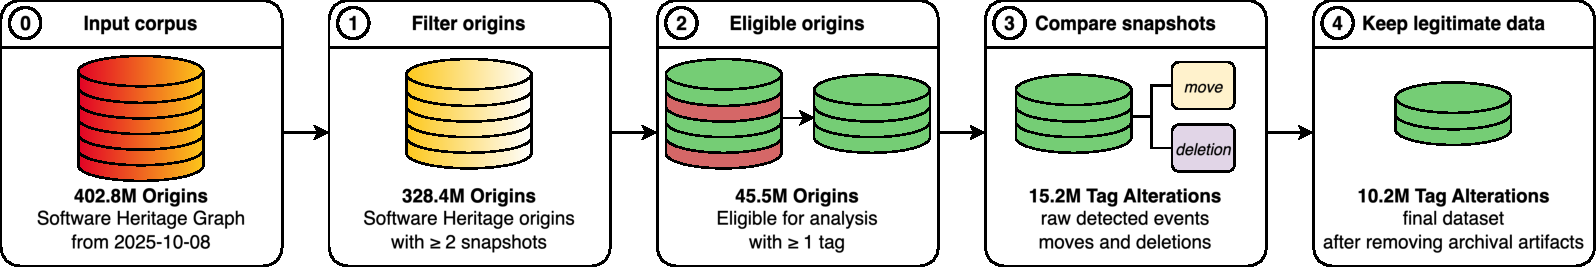
\includegraphics[width=0.74\linewidth]{workflow_pipeline.drawio.pdf}
    \end{center}
\end{frame}
\fi
% --- END CUT ---

% ------------------------------------------------------------------
\begin{frame}{Scale: tag alterations are not anecdotal}
    \sidefigbegin
    \begin{columns}[T,totalwidth=\linewidth]
        \begin{column}{0.36\linewidth}
            \begin{itemize}
                \item \textbf{\TotalAlterationsShort{}} alterations (\TemporalSpan),
                      \AlteredRepositoriesShort{} repos
                      (\AlteredRepositoriesPercent{} of tagged
                      origins)~\cite{rapaport2026tagalterations}.
                \item \textbf{Lower bound} (gaps between archival visits);
                      persistent over time, not a one-off spike.
                \item \textbf{Deletions} \DeletionsShort{} (\DeletionsPercent):
                      hurt \emph{availability} (fail loud).
                \item \textbf{Moves} \LegitMovesShort{} (\LegitMovesPercentOfAlterations):
                      hurt \emph{integrity} (fail silent).
            \end{itemize}
        \end{column}
        \begin{column}{0.64\linewidth}
            \begin{center}
                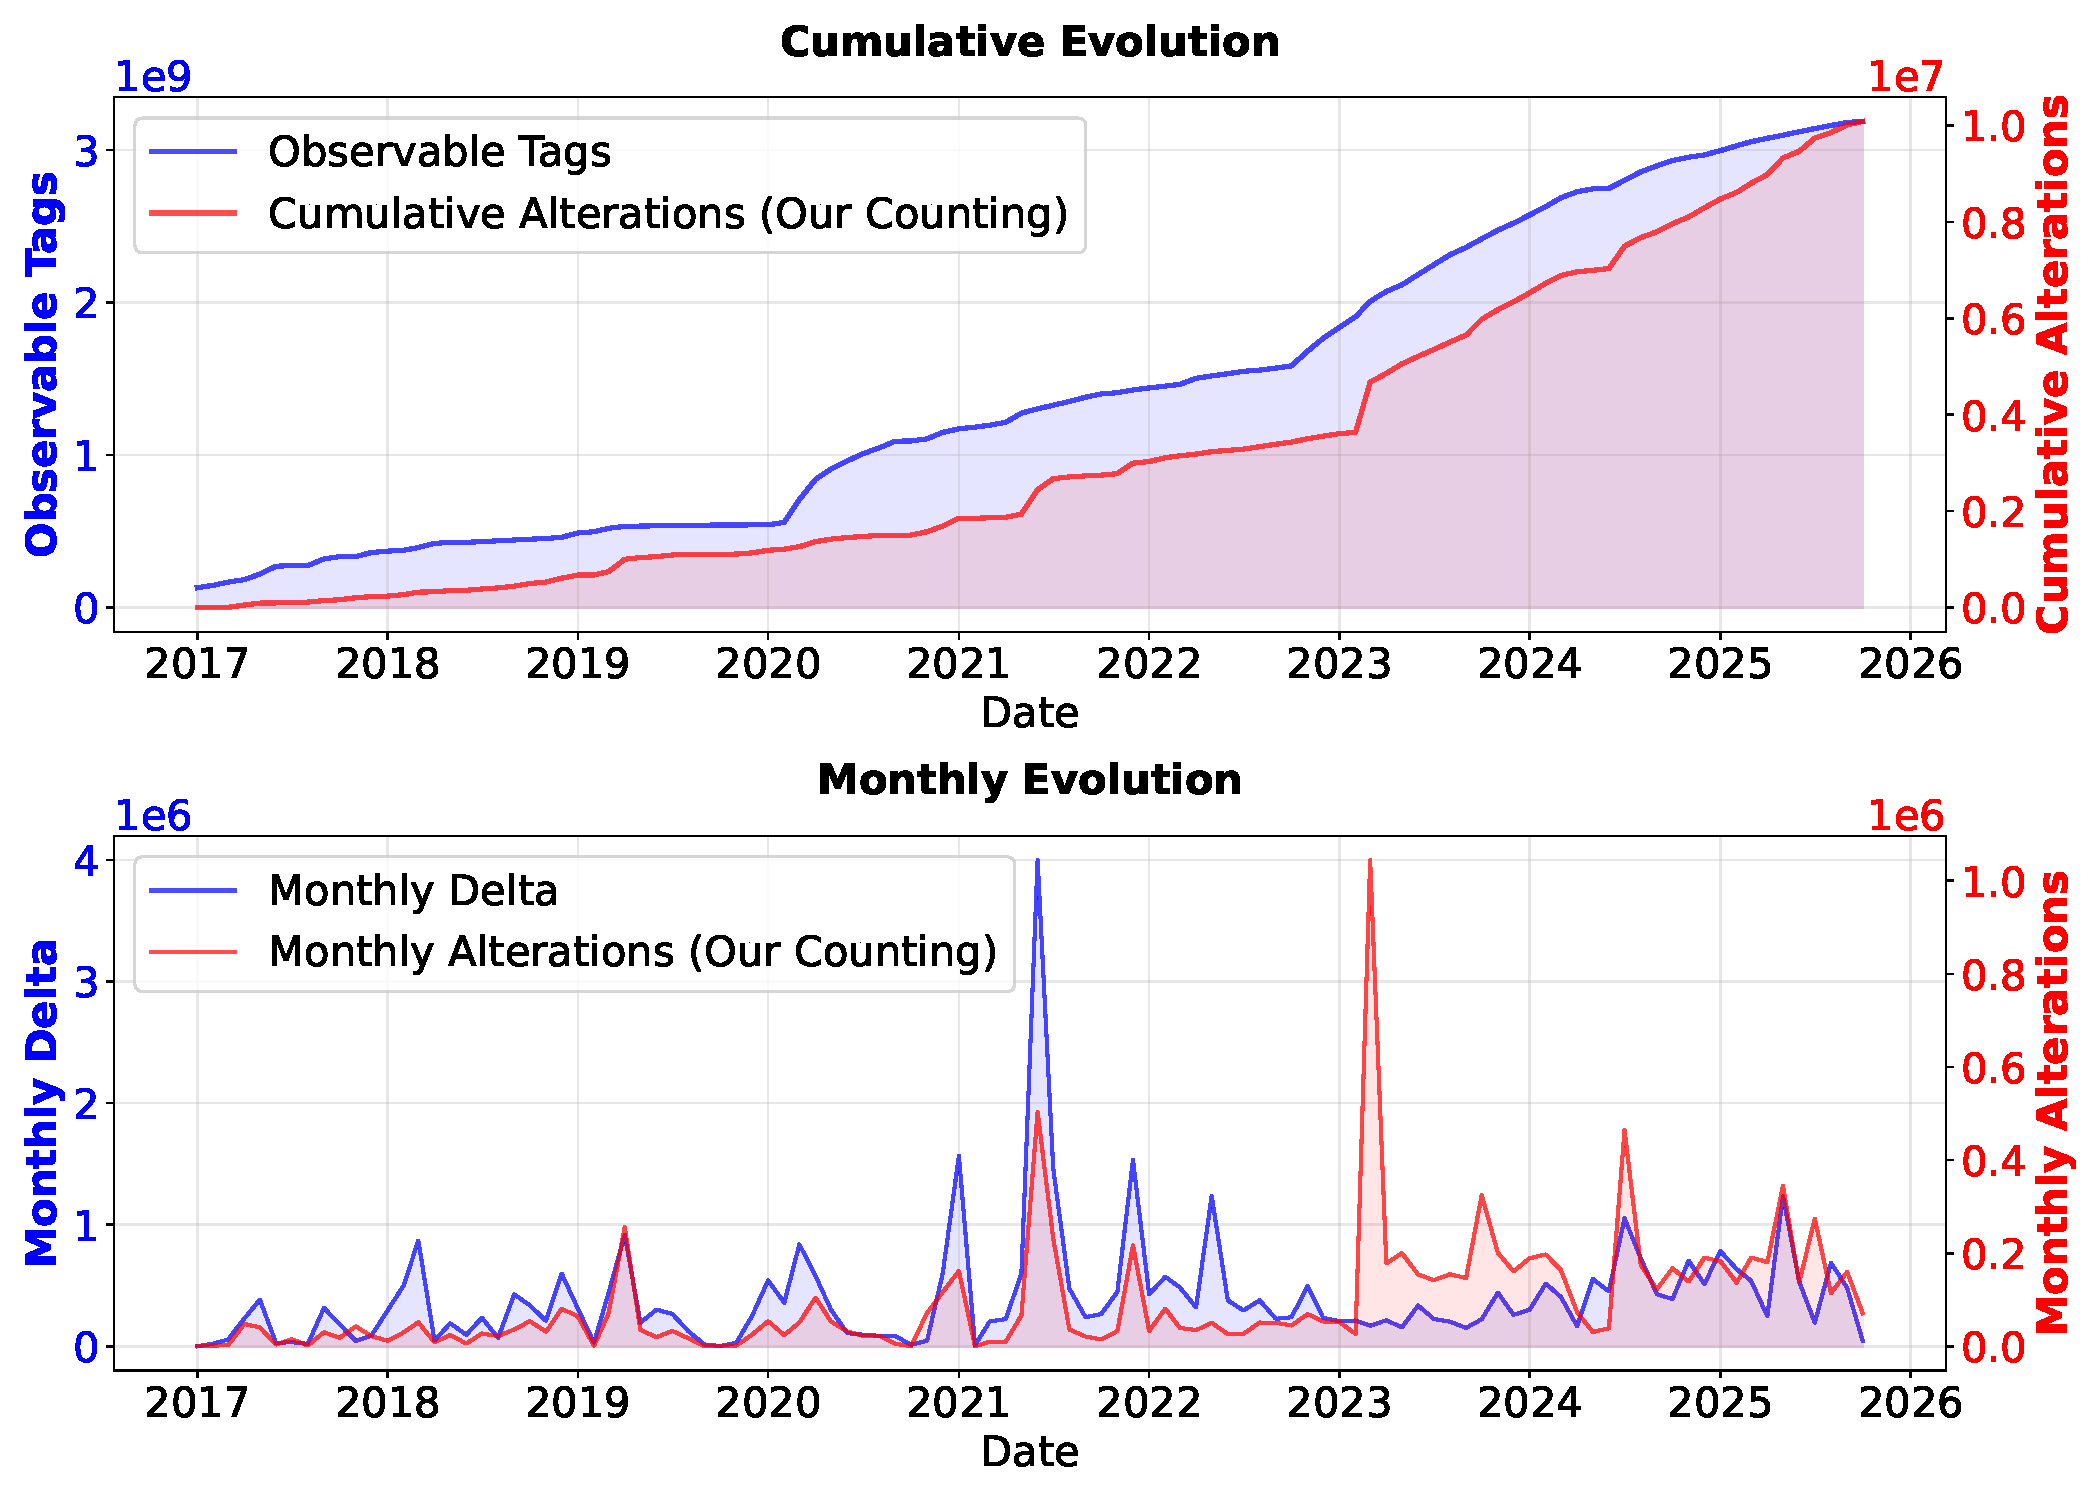
\includegraphics[width=1.05\linewidth]{temporal_evolution.pdf}
            \end{center}
        \end{column}
    \end{columns}
    \sidefigend
\end{frame}

% ------------------------------------------------------------------
\begin{frame}[c]{Taxonomy: what kind of change is a ``move''?}
    \sidefigbegin
    \begin{columns}[c,totalwidth=\linewidth]
        \begin{column}{0.39\linewidth}
            \begin{itemize}
                \item Deletions mainly threaten \emph{availability}.
                \item Moves keep the label, change its meaning.
                \item \textbf{\PercentMovesContentChange{} of moves
                      change source-tree content}
                      (\MovesWithContentChangeShort{})---not just metadata.\\
                      $\Rightarrow$ threaten \emph{integrity}.
            \end{itemize}
            \vspace{2em}
        \end{column}
        \begin{column}{0.59\linewidth}
            \includegraphics[width=\linewidth,height=\textheight,keepaspectratio]{taxonomy.pdf}
        \end{column}
    \end{columns}
    \sidefigend
\end{frame}

% ------------------------------------------------------------------
\begin{frame}[c]{Popularity: not just obscure repositories}
    \sidefigbegin
    \begin{columns}[T,totalwidth=\linewidth]
        \begin{column}{0.37\linewidth}
            \vspace{1em}
            \begin{itemize}
                \item \textbf{Volume:}\\\StarZeroOneAlterationsPercent{} of alterations in 0--1 star repos.
                \item \textbf{Prevalence:}\\$P(\geq 1$ alteration$)$ rises with stars:\\
                      \small{\StarPropZeroOnePctTrunc{} (0--1) $\rightarrow$ \StarPropFiveHundredPlusPctTrunc{} (501+).}
                \item Popularity does \textbf{not} protect against tag alterations ---
                      though stars are an imperfect, gameable
                      proxy~\cite{borges-2016-github-stars,DBLP:journals/corr/abs-2412-13459}.
            \end{itemize}
        \end{column}
        \begin{column}{0.6\linewidth}
            \begin{center}
                \includegraphics[width=\linewidth,height=0.86\textheight,keepaspectratio]%
                                {popularity_proportion.pdf}
            \end{center}
        \end{column}
    \end{columns}
    \sidefigend
\end{frame}

% ------------------------------------------------------------------
% ------------------------------------------------------------------
\begin{frame}[fragile]{Impact: coordinated retargeting, and Nixpkgs already fails}
    % \sidefigbegin
    % \begin{columns}[T,totalwidth=\linewidth]
    %     \begin{column}{0.48\linewidth}
    %         \small
            \begin{itemize}
                \item Fork \AttackRepoFork{}: \AttackTagMovesCount{} tags moved to \textbf{one} malicious revision.
                \item Nix pins by fixed-output hash~\cite{DBLP:conf/lisa/DolstraJV04}:
                      \NixPkgsTracked{} packages in our altered-tag set;
                      \NixPkgsHashMismatch{} confirmed rebuild failures
                      (\NixPkgsFailDeletion{} deletion, \NixPkgsFailHashMismatch{} hash mismatch).
            \end{itemize}
            \vspace{0.3em}
            \begin{terminalbox}
$ nix build ...#libv3270.src --rebuild
error: hash mismatch:
  specified: sha256-...
  got:       sha256-...
            \end{terminalbox}
            % \vspace{0.4em}
            % {\small Tag \emph{names} are not stable anchors: record the
            %  \textbf{commit / content hash}. Not every alteration is malicious.}
    %     \end{column}
    %     \begin{column}{0.50\linewidth}
    %         \centering
    %         \includegraphics[width=\linewidth,height=0.72\textheight,keepaspectratio]{fig_attack_retarget.pdf}
    %     \end{column}
    % \end{columns}
    % \sidefigend
\end{frame}

% --- CUT: merged into Impact (attack + Nixpkgs) ---
\iffalse
\begin{frame}{Threat: delayed retargeting in a real attack}
    \begin{itemize}
        \item Fork \AttackRepoFork{} (related to \texttt{tj-actions/changed-files}).
        \item \AttackTagMovesCount{} tags simultaneously moved to the \textbf{same} malicious revision.
        \item Consumers who ``pinned'' \texttt{v39} to \texttt{v47} got new code on the next fetch.
        \item \AttackStableCases{} tags had been stable $\geq\AttackStableDaysLowerBound{}$ days---trusted pins, not fresh noise.
    \end{itemize}
\end{frame}

\begin{frame}[fragile]{Threat: Nixpkgs already sees the failures}
    \begin{itemize}
        \item Nix pins sources by fixed-output hash~\cite{DBLP:conf/lisa/DolstraJV04}:
              \NixPkgsTracked{} packages reference origins in our altered-tag dataset;\\
              \NixPkgsAffected{} altered tags appear in recipes.
        \item \NixPkgsHashMismatch{} confirmed rebuild failures without binary cache:
              \NixPkgsFailDeletion{} tag deleted (availability);
              \NixPkgsFailHashMismatch{} hash mismatch after retargeting (integrity).
    \end{itemize}
    \vspace{0.4em}
    \begin{lstlisting}[basicstyle=\ttfamily,breaklines=true,frame=single]
$ nix build ...#libv3270.src --rebuild --no-link --impure -L
error: hash mismatch in fixed-output derivation '...':
         specified: sha256-...
            got:    sha256-...
    \end{lstlisting}
\end{frame}
\fi
% --- END CUT ---

% --- CUT: takeaway folded into Impact ---
\iffalse
\begin{frame}{Study 1 --- conclusion}
    \begin{itemize}
        \item Tag \emph{names} are useful for humans; they are \textbf{not} stable dependency anchors.
        \item At scale: deletions hurt availability; most moves change \textbf{actual content}.
        \item For builds and research: record the \textbf{commit / content hash} (or SWHID)
              alongside any human-readable tag---tag alone is
              insufficient~\cite{github_secure_use_third_party_actions}.
        \item Platforms: audit tag create/move/delete; ``immutable
              releases''~\cite{github_immutable_releases} help but are
              \textbf{opt-in}, Releases-only, and forge-specific.
        \item We do \textbf{not} claim every alteration is malicious---only that mutable names and time-invariant references are in tension.
    \end{itemize}
\end{frame}
\fi
% --- END CUT ---

%##############################################################################
\section{Study 2: Altered Histories}
%##############################################################################

% ------------------------------------------------------------------
% [feedback] Less abrupt opening: history rewriting is a USEFUL feature first.
\begin{frame}[fragile]{History rewriting is a feature --- before it is a risk}
    \begin{terminalbox}
        $ git rebase --interactive <...>
        $ git push --force
    \end{terminalbox}
    \vspace{0.2em}
    \begin{columns}[T,totalwidth=\textwidth]
        \begin{column}{0.58\textwidth}
            \small
            \begin{itemize}
                \item \textbf{Legitimate use:} clean up your work \emph{before} sharing ---
                      squash, reorder, fix typos --- normally done before code stabilises
                      in a production branch~\cite{DBLP:journals/ese/GermanAH16}.
                \item \textbf{The catch:} the same feature lets you rewrite a
                      \textbf{production branch} (\texttt{main}, \texttt{master}), breaking
                      workflows, reproducibility, and supply-chain assumptions.
            \end{itemize}
        \end{column}
        \begin{column}{0.42\textwidth}
            \centering
            \includegraphics[width=0.82\linewidth,height=0.4\textheight,keepaspectratio]{big_brother.jpeg}
        \end{column}
    \end{columns}
\end{frame}

% --- CUT: duplicate of Method (SWH as independent witness) ---
\iffalse
% [feedback] Winners' history + SWH as the archive that preserves the real past.
\begin{frame}{You only see the version of the winners}
    \begin{itemize}
        \item On a forge like GitHub you only ever see the \textbf{official} history ---
              the one that was rewritten. ``History is written by the winners.''
        \item \textbf{Software Heritage} continuously indexes as many versions of software as
              possible, preserving history \textbf{as it really was}.
        \item That independent record is what lets us ask: were these rewrites \emph{justified},
              or did they \textbf{hide something} (security holes, awkward past states)?
    \end{itemize}
    \vspace{0.4em}
    {\small We detect and classify the rewrites; the archive is what makes the vanished past observable again.}
\end{frame}
\fi
% --- END CUT ---

% ------------------------------------------------------------------
\begin{frame}{Method and scale: detecting rewritten histories}
    \sidefigbegin
    \centering
    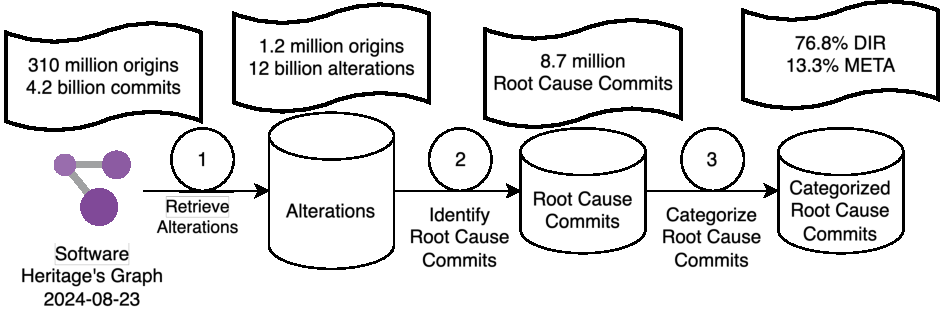
\includegraphics[width=\linewidth,height=0.52\textheight,keepaspectratio]{flowchart.drawio.pdf}
    \vspace{0.35em}
    \begin{columns}[T,totalwidth=\linewidth]
        \begin{column}{0.48\linewidth}
            \small
            \raggedright
            \begin{itemize}
                \item Compare successive SWH snapshots of
                      \textbf{\OriginsTwoVisitsOrMoreShort{}} Git origins.
                \item Isolate \textbf{root-cause} commits from snowball-propagated descendants.
            \end{itemize}
        \end{column}
        \begin{column}{0.48\linewidth}
            \small
            \raggedright
            \begin{itemize}
                \item \textbf{\GitOriginsRootCauseCommitsShort{}} repositories
                      (\textasciitilde\PercentOriginsAltered{}) with
                      \textbf{\GitRootCauseCommitsShort{}} root-cause
                      commits~\cite{DBLP:conf/kbse/RapaportPTZ25}.
                \item Same popularity gradient as Study~1:
                      \StarAlterRateZeroOne{} (0--1 stars) $\rightarrow$
                      \StarAlterRateThousandPlus{} (1000+).
            \end{itemize}
        \end{column}
    \end{columns}
    \sidefigend
\end{frame}

% --- CUT: merged into ``Method and scale'' ---
\iffalse
\begin{frame}{Methodology}
    \vfill
    \begin{columns}[T,totalwidth=\textwidth]
        \begin{column}{0.5\textwidth}
            \begin{itemize}
                \item \textbf{Software Heritage} archive --- avoids the classic
                      single-forge mining pitfalls~\cite{bird2009promisesmininggit,kalliamvakou2014promises}
                \item Extract all Git repositories
                      \begin{itemize}
                          \item \textbf{\OriginsTwoVisitsOrMoreShort{} Git repositories}
                      \end{itemize}
                \item Compare snapshots to detect altered commits
                \item Isolate \textbf{root causes} from snowball-propagated changes
                \item Classify altered commits
            \end{itemize}
        \end{column}
        \begin{column}{0.5\textwidth}
            \centering
            \includegraphics[width=0.9\linewidth]{swh-without-time-slides.drawio.pdf}
        \end{column}
    \end{columns}
\end{frame}

\begin{frame}{How often are histories altered?}
    \begin{itemize}
        \item \textbf{\GitOriginsRootCauseCommitsShort{} repositories} with observable
              altered histories (\textasciitilde\PercentOriginsAltered{} of
              origins with $\geq 2$ visits)~\cite{DBLP:conf/kbse/RapaportPTZ25}.
        \item \textbf{\GitRootCauseCommitsShort{}} root-cause commits --- the edits that
              start a rewrite, after peeling off snowball-propagated descendants.
        \item Absolute volume is large even at a modest rate: many developers interact with
              rewritten public history.
        \item No prior large-scale measurement existed; altered history is designed to
              \textbf{disappear} from the forge, so the archive is what makes the count possible.
    \end{itemize}
\end{frame}
\fi
% --- END CUT ---

% ------------------------------------------------------------------
\begin{frame}{Where alterations land: branch distribution}
    \sidefigbegin
    \begin{columns}[T,totalwidth=\linewidth]
        \begin{column}{0.42\linewidth}
            \small
            \begin{itemize}
                \item Pull-request branches: \textbf{37.6\%} --- legitimate cleanup
                      before merge.
                \item \emph{Renovate} bot branches: \textbf{9.6\%} --- rewriting is inherent
                      to automated dependency updates.
                \item But \texttt{main}/\texttt{master}: \textbf{11.4\%} --- 2nd most affected
                      category, and the one consumers and auditors trust.
                \item Development branches: \textbf{0.9\%} --- rarer, but still disruptive
                      when shared.
            \end{itemize}
        \end{column}
        \begin{column}{0.56\linewidth}
            \centering
            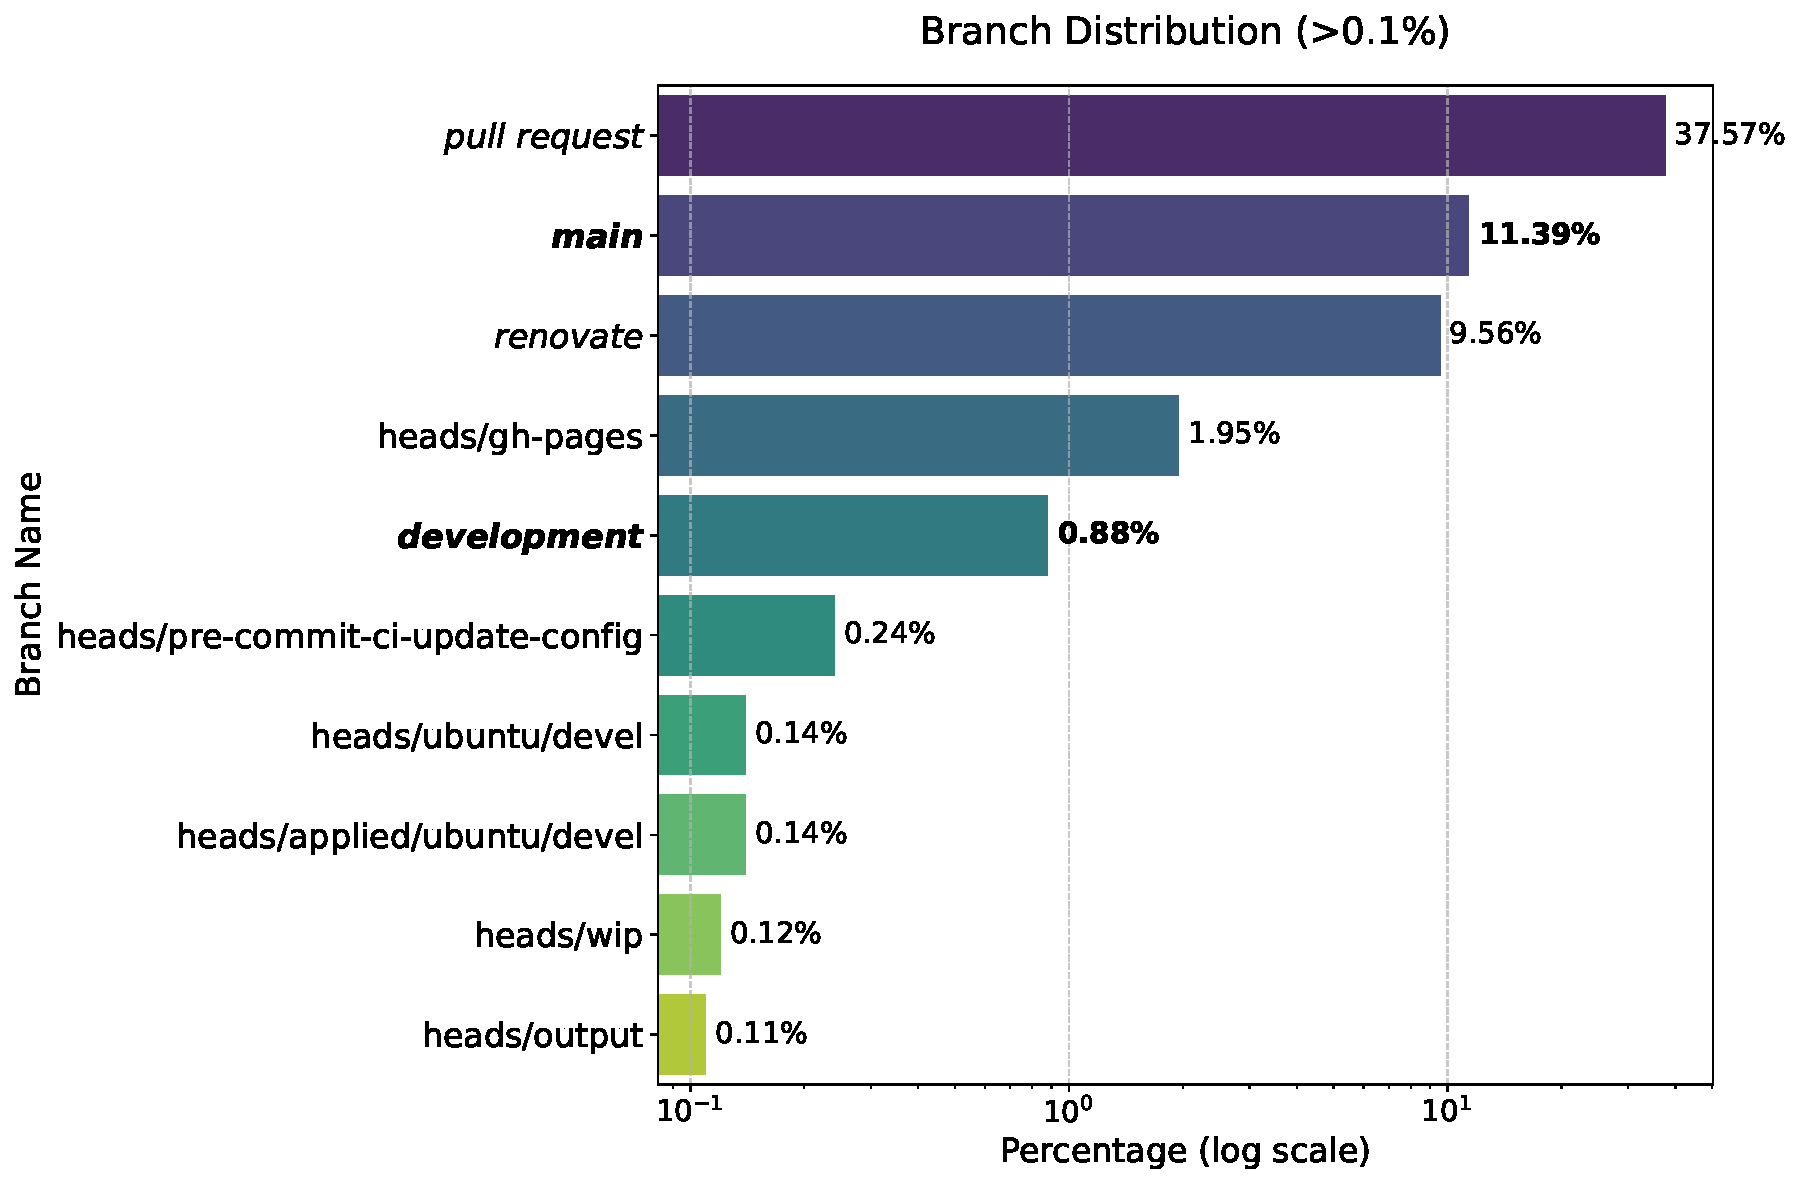
\includegraphics[width=1.05\linewidth,height=0.85\textheight,keepaspectratio]{distrib_branch.pdf}
        \end{column}
    \end{columns}
    \sidefigend
\end{frame}

% ------------------------------------------------------------------
% --- CUT: same popularity lesson as Study 1; spoken on method+scale ---
\iffalse
\begin{frame}{Which repositories? Popularity does not protect}
    \sidefigbegin
    \begin{columns}[T,totalwidth=\linewidth]
        \begin{column}{0.42\linewidth}
            \small
            \begin{itemize}
                \item Gradient across star buckets:
                      \begin{itemize}
                          \item 0--1 stars: \StarAlterRateZeroOne{} alteration rate
                          \item 1000+ stars: \StarAlterRateThousandPlus{} alteration rate
                      \end{itemize}
                \item \textbf{More popular $\Rightarrow$ more often altered} --- mature,
                      high-visibility projects are more likely to rewrite history.
                \item Absolute volume still sits in the long tail, but prevalence rises with
                      stars (same pattern as Study~1 on tags).
            \end{itemize}
        \end{column}
        \begin{column}{0.56\linewidth}
            \centering
            \includegraphics[width=\linewidth,height=0.82\textheight,keepaspectratio]%
                            {proportion_res_stars.pdf}
        \end{column}
    \end{columns}
    \sidefigend
\end{frame}
\fi
% --- END CUT ---

% ------------------------------------------------------------------
\begin{frame}{What changed: category taxonomy}
    \sidefigbegin
    \begin{columns}[T,totalwidth=\linewidth]
        \begin{column}{0.42\linewidth}
            \small
            \begin{itemize}
                \item \textbf{Directory / content} changes dominate
                      (\PercentDIRRootCauseCommits):
                      \begin{itemize}
                          \item File modified: \PercentCategFileModified
                          \item File removed: \PercentCategFileRemoved
                          \item Content split: \PercentCategContentSplit
                      \end{itemize}
                \item \textbf{Metadata-only} rewrites (\PercentMETARootCauseCommits):
                      author, committer, dates, messages --- committer date alone
                      \PercentCategCommitterDate~\cite{torresarias2016gitmetadata}.
                \item The profile of \textbf{1000+ star} repositories matches the whole corpus.
            \end{itemize}
        \end{column}
        \begin{column}{0.56\linewidth}
            \centering
            \vspace{2em}
            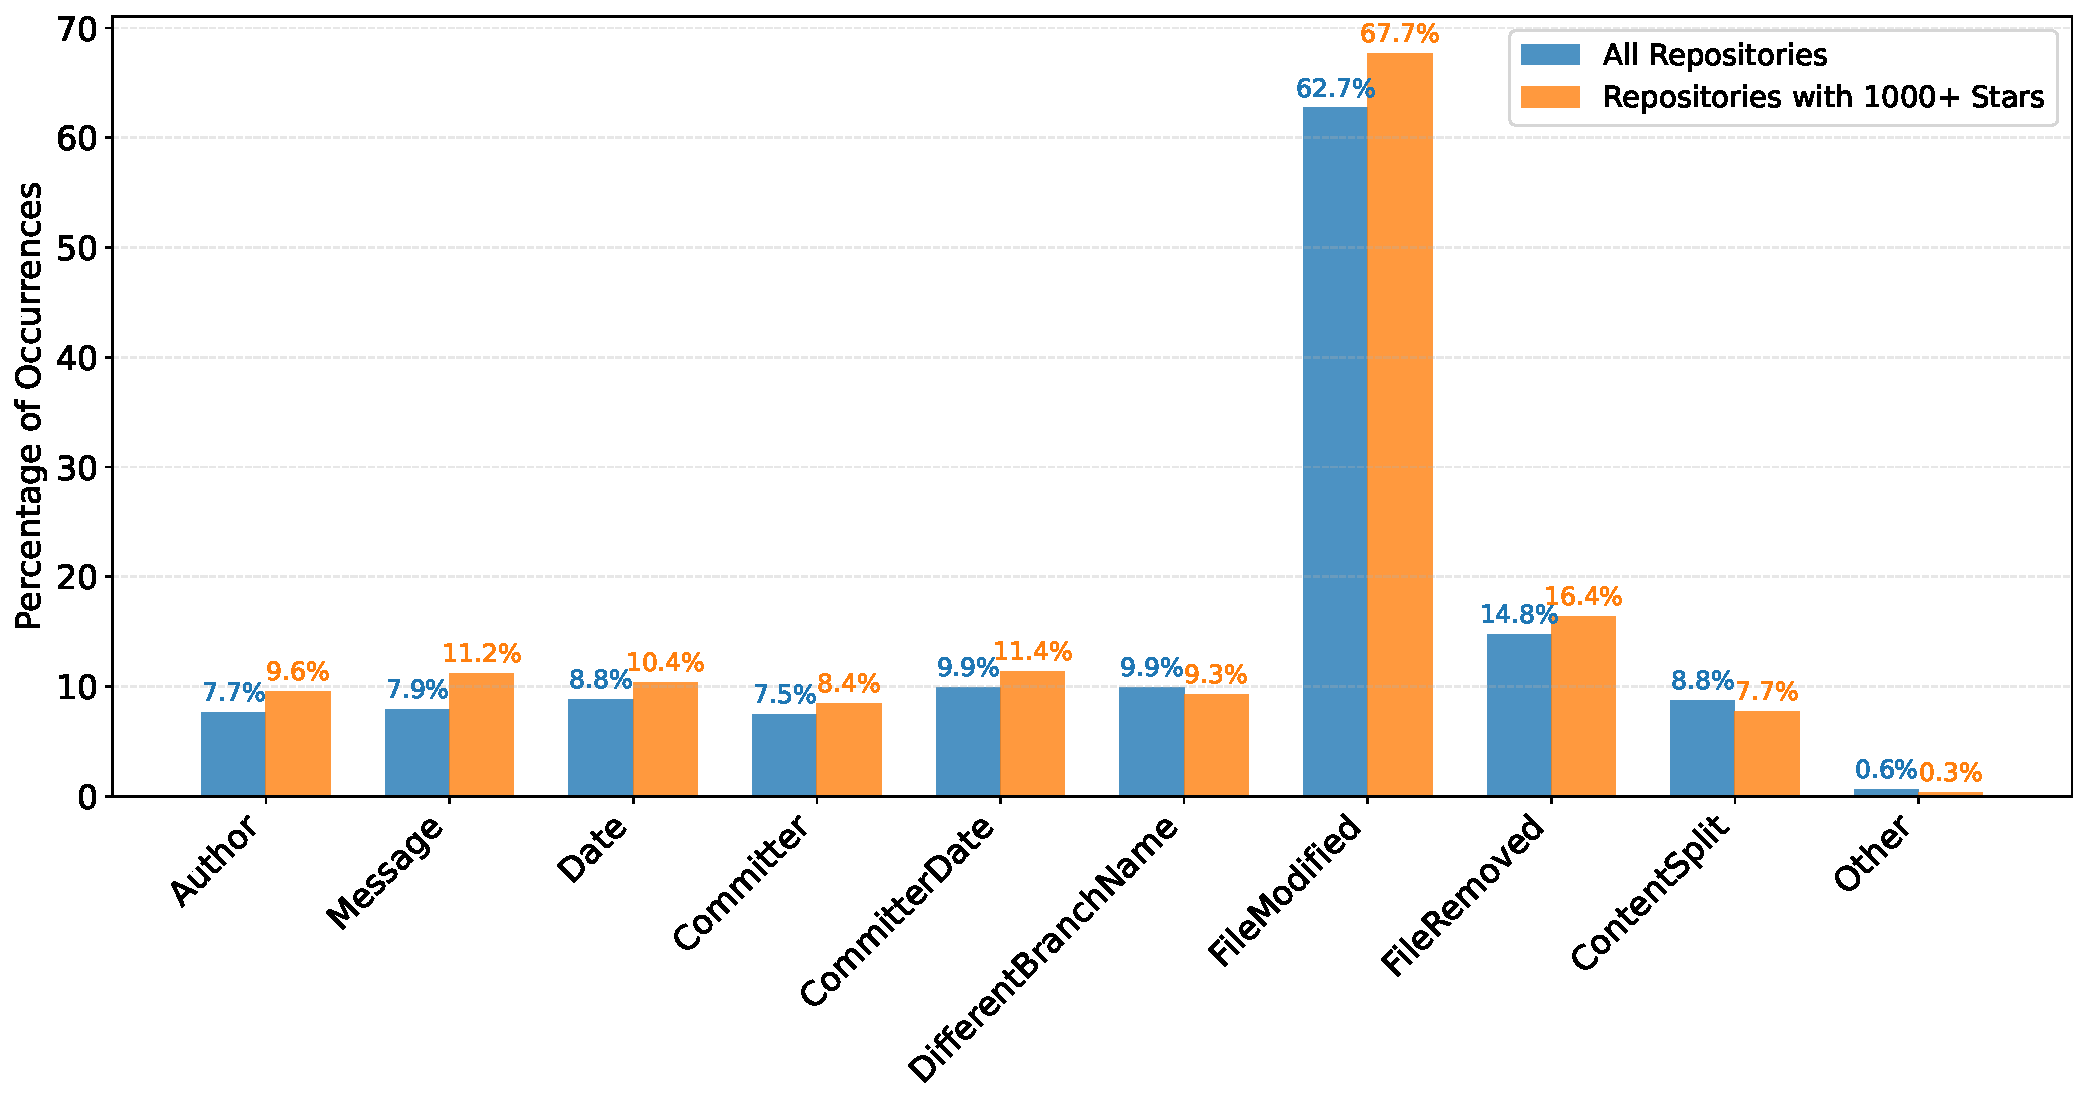
\includegraphics[width=1.05\linewidth,height=\textheight,keepaspectratio]{distrib_categ.pdf}
        \end{column}
    \end{columns}
    \sidefigend
\end{frame}

% ------------------------------------------------------------------
% --- CUT: LICENSE at #20 mentioned on the case-study slide ---
\iffalse
\begin{frame}{File patterns in alterations}
    \begin{columns}[T,totalwidth=\textwidth]
        \begin{column}{0.58\textwidth}
            \centering
            \scriptsize
            \setlength{\tabcolsep}{3pt}%
            \begin{tabular}{@{}rlr@{\hspace{1.2em}}rlr@{}}
                \toprule
                \textbf{\#} & \textbf{File} & \textbf{Count} &
                \textbf{\#} & \textbf{File} & \textbf{Count} \\
                \midrule
                1  & \path{default.nix}    & 13.4\,M & 11 & \path{CHANGELOG.md}   & 5.0\,M \\
                2  & \path{package.json}   & 12.6\,M & 12 & \path{__init__.py}& 4.9\,M \\
                3  & \path{Makefile}       & 10.6\,M & 13 & \path{metadata.xml}   & 4.5\,M \\
                4  & \path{README.md}      & 10.0\,M & 14 & \path{CMakeLists.txt} & 4.4\,M \\
                5  & \path{index.js}       & 9.1\,M  & 15 & \path{package.py}     & 4.3\,M \\
                6  & \path{Manifest}       & 8.9\,M  & 16 & \path{APKBUILD}       & 3.4\,M \\
                7  & \path{pom.xml}        & 7.1\,M  & 17 & \path{template}       & 3.1\,M \\
                8  & \path{index.html}     & 6.3\,M  & 18 & \path{BUILD}          & 3.0\,M \\
                9  & \path{meta.yaml}      & 5.4\,M  & 19 & \path{index.ts}       & 2.8\,M \\
                10 & \path{index.md}       & 5.4\,M  & 20 & \path{LICENSE}        & 2.8\,M \\
                \bottomrule
            \end{tabular}
        \end{column}
        \begin{column}{0.40\textwidth}
            \begin{itemize}
                \item Build / packaging configs dominate:
                      \texttt{default.nix}, \texttt{package.json}, \texttt{Makefile}.
                \item Documentation: \texttt{README.md}, \texttt{CHANGELOG.md}.
                \item Notable: \texttt{LICENSE} at rank \#20 --- leads into the licence
                      case study.
            \end{itemize}
        \end{column}
    \end{columns}
\end{frame}
\fi
% --- END CUT ---

% ------------------------------------------------------------------
% ------------------------------------------------------------------
\begin{frame}{Two case studies: licences and secrets}
    \begin{columns}[T,totalwidth=\textwidth]
        \begin{column}{0.48\textwidth}
            \small
            \textbf{Licences --- rewriting the past}
            \begin{itemize}
                \item \LicenseAllShort{} altered license files on \textbf{main};
                      \LicenseOrigins{} repositories (\texttt{LICENSE} is rank \#20 among altered files).
                \item ScanCode~\cite{scancode-home}:
                      \LicenseUpdate{} version updates,
                      \LicenseFullChange{} full changes,
                      \LicensePartialChange{} partial.
                \item Retroactive rewrite: as if the \emph{new} license had always been the only valid one --- rights already granted may disappear.
            \end{itemize}
        \end{column}
        \begin{column}{0.50\textwidth}
            \small
            \textbf{Secrets --- bridge to Study 3}
            \begin{itemize}
                \item \SecretsRemovedAllShort{} secret-looking file removals,
                      \SecretsOriginsAllShort{} repositories.
                \item \textbf{Removal $\neq$ security:} clones and archives persist.
                \item Keys must be \textbf{rotated} at the provider.
                \item Study~3 recovers the content and checks what those files held.
            \end{itemize}
        \end{column}
    \end{columns}
\end{frame}

% --- CUT: merged into ``Two case studies'' ---
\iffalse
\begin{frame}{Case study 1: license changes --- rewriting the past}
    \begin{itemize}
        \item \textbf{\LicenseAllShort{}} altered license files on \textbf{main} branches;
              \LicenseOrigins{} repositories (\LicenseOriginsThousandPlus{} with 1000+ stars).
        \item Licences identified with ScanCode~\cite{scancode-home}:
              \begin{itemize}
                  \item \LicenseUpdate{} version updates (e.g.\ GPL-2 $\rightarrow$ GPL-3)
                  \item \LicenseFullChange{} full changes (MIT $\rightarrow$ GPL)
                  \item \LicensePartialChange{} partial edits
              \end{itemize}
        \item \textbf{The 1984 parallel:} a retroactive rewrite tries to make it look as if
              the \emph{new} license was always the only valid one.
        \item \textbf{Legal concern:} retroactively changing a license may remove
              rights that were already granted.
    \end{itemize}
\end{frame}

\begin{frame}{Case study 2: removing secrets (bridge to Study 3)}
    \begin{itemize}
        \item \textbf{\SecretsRemovedAllShort{}} file removals whose names suggest secrets
              (private keys, certificates, passwords), across \SecretsOriginsAllShort{}
              repositories.
        \item \textbf{Removal $\neq$ security:} archived and cloned copies persist.
        \item Keys must be \textbf{rotated} at the provider, not only purged from Git.
        \item A security signal of risky operational practice --- and exactly where
              \textbf{Study 3} begins: recover the content and check what those files
              really held.
    \end{itemize}
\end{frame}
\fi
% --- END CUT ---

% ------------------------------------------------------------------
\begin{frame}[fragile]{GitHistorian: making the archive queryable}
    \begin{columns}[T,totalwidth=\textwidth]
        \begin{column}{0.42\textwidth}
            \small
            \begin{itemize}
                \item Open-source detection of history alterations, with categorisation and CI/CD hooks.\footnote[frame]{\url{https://github.com/srapaport/git-historian}}
                \item Replication package~\cite{replication-package-altered-histories}.
            \end{itemize}
            \vspace{0.5em}
            {\small\textbf{Takeaway:} \GitOriginsRootCauseCommitsShort{} repositories,
             11.4\% of alterations on \texttt{main}/\texttt{master};
             protect production branches and treat rewritten history as a visibility gap.}
        \end{column}
        \begin{column}{0.56\textwidth}
            \begin{terminalboxsmall}
$ git-historian check \
    github.com/example/project --verbose
Connected to the database!
Found 2 altered history records.

Record #1:
  Branch:   refs/heads/master
  Altered:  swh:1:rev:a1b2c3d4...
  Snapshot: swh:1:snp:abcd1234...
  Category: FileModified

Saved to ~/.local/state/git-historian/
            \end{terminalboxsmall}
        \end{column}
    \end{columns}
\end{frame}

% --- CUT: takeaway folded into GitHistorian ---
\iffalse
\begin{frame}{Study 2 --- conclusion}
    \begin{itemize}
        \item First large-scale measurement: \GitOriginsRootCauseCommitsShort{} repositories,
              \GitRootCauseCommitsShort{} root-cause commits.
        \item \textbf{11.4\%} of alterations land on \texttt{main}/\texttt{master}; popularity
              does \textbf{not} protect.
        \item Content changes dominate; recurring targets include build configs, docs, and
              \texttt{LICENSE}.
        \item Two critical case studies: \textbf{licences} (retroactive rights risk) and
              \textbf{secrets} (removal without revocation).
        \item Practice: protect production branches; make automated auditing routine;
              treat rewritten history as a supply-chain visibility gap.
        \item \textbf{GitHistorian} turns the archival witness into a queryable check.
    \end{itemize}
\end{frame}
\fi
% --- END CUT ---

%##############################################################################
\section{Study 3: Removed Secrets}
%##############################################################################

% ------------------------------------------------------------------
\begin{frame}{Removal is not revocation}
    \begin{itemize}
        \item Hard-coded credentials leak at scale and are a long-standing weakness
              class~\cite{DBLP:conf/ndss/MeliMR19,segura2022secrets,cwe798}.
        \item After a leak, two actions are \textbf{not interchangeable}~\cite{DBLP:journals/corr/abs-2211-06213}:
              \begin{itemize}
                  \item \textbf{Cleanup} (optional) --- rewrite the repo (amend/rebase, force-push) so the
                        current view no longer shows the file. \emph{Visible, easy.}
                  \item \textbf{Rotation} (mandatory) --- revoke/replace the credential at the provider that
                        issued it. \emph{The only thing that invalidates a
                        leak}~\cite{DBLP:conf/secdev/BasakNRW22}.
              \end{itemize}
        \item Cleanup is easy to mistake for rotation, and an archive can't see rotation ---
              but it \textbf{can} show whether erased secrets remain \textbf{recoverable}.
        \item Do the secrets developers tried to erase still sit in the archive?
    \end{itemize}
\end{frame}

% ------------------------------------------------------------------
% ------------------------------------------------------------------
\begin{frame}{Detection funnel: from altered files to findings}
    \begin{columns}[c,totalwidth=\textwidth]
        \begin{column}{0.62\textwidth}
            \centering
            \begin{tikzpicture}[
                funnel/.style={draw=tptred, line width=0.8pt, rounded corners=2pt,
                               align=center, inner sep=5pt, font=\small}
            ]
                \node[funnel, minimum width=0.95\linewidth, fill=tptred!12] (f1)
                    {\textbf{\SecretFirstExtractionShort{}} broad filename matches};
                \node[funnel, minimum width=0.82\linewidth, fill=tptred!8, below=5pt of f1] (f2)
                    {\textbf{\SecretSecondExtractionShort{}} refined names ($\approx 128{:}1$)};
                \node[funnel, minimum width=0.68\linewidth, fill=tptred!5, below=5pt of f2] (f3)
                    {\textbf{\SecretResolvedBlobs{}} unique recoverable blobs};
                \node[funnel, minimum width=0.55\linewidth, fill=tptred!18, below=5pt of f3] (f4)
                    {\textbf{\SecretFindingBlobs{}} blobs with $\geq 1$ finding
                     \quad(\SecretDetectionRate)};
            \end{tikzpicture}
        \end{column}
        \begin{column}{0.36\textwidth}
            \small
            \begin{itemize}
                \item Start from Study~2 altered files.
                \item Recover from SWH, deduplicate, scan (gitleaks + TruffleHog).
                \item Filename signal: \texttt{id\_rsa} 81\% vs.\ \texttt{.py} 1.5\%.
            \end{itemize}
        \end{column}
    \end{columns}
\end{frame}

% --- CUT: replaced by funnel figure ---
\iffalse
\begin{frame}{A staged detection pipeline (recall $\to$ precision)}
    \begin{enumerate}
        \item \textbf{Start} from altered files in Study 2 --- far too many to scan directly.
        \item \textbf{Broad filename pass} (high recall): whole extension classes that
              \emph{could} hide a secret $\to$ \SecretFirstExtractionShort{} records.
        \item \textbf{Refined filename pass} (precision): only basenames that themselves look
              like credentials $\to$ \SecretSecondExtractionShort{} candidates ($\approx128{:}1$).
        \item \textbf{Recover} archived content from SWH; \textbf{deduplicate} identical blobs.
        \item \textbf{Scan} with two detectors (gitleaks + TruffleHog), whose complementary
              precision is documented~\cite{DBLP:conf/msr/BasakNRW23,DBLP:conf/esem/BasakCRW23}.
        \item \textbf{Link} each finding back to \emph{every} repository location sharing that blob.
    \end{enumerate}
\end{frame}

\begin{frame}{Detection funnel: candidates $\to$ findings}
    \begin{center}
    \small
    \begin{tabular}{lr}
        \toprule
        \textbf{Stage} & \textbf{Count} \\
        \midrule
        First (broad) filename selection      & \num{365591843} \\
        Refined filename selection            & \num{2846017} \\
        \midrule
        Locations resolved to archived content & \num{2187481} \\
        Unresolved candidate locations         & \num{658536} \\
        Unique recoverable content blobs       & \num{281740} \\
        Downloaded blobs                       & \num{281728} \\
        \textbf{Blobs with $\geq 1$ finding}   & \textbf{\num{25859}} \\
        Overall blob-level detection rate      & \SI{9.18}{\percent} \\
        \bottomrule
    \end{tabular}
    \end{center}
\end{frame}
\fi
% --- END CUT ---

% ------------------------------------------------------------------
% ------------------------------------------------------------------
\begin{frame}{What we found: recoverable secrets, mostly well-formed keys}
    \begin{columns}[T,totalwidth=\textwidth]
        \begin{column}{0.52\textwidth}
            \small
            \begin{itemize}
                \item \SecretDetectionRate{} of recovered blobs still look like secrets
                      (\SecretFindingBlobs{} of \SecretResolvedBlobs).
                \item \textbf{Private keys dominate} both detector rankings.
                \item Offline parse (Tier~A): \SecretPKValidBlobs{} of
                      \SecretPKFlaggedBlobs{} gitleaks private-key blobs are
                      \textbf{cryptographically valid} (\SecretPKValidPct).
                \item Syntactic validity $\neq$ still active --- a revoked key still parses.
            \end{itemize}
        \end{column}
        \begin{column}{0.46\textwidth}
            \centering
            \begin{tikzpicture}[
                box/.style={draw=tptred, line width=0.8pt, rounded corners=2pt,
                            align=center, inner sep=7pt, font=\small, minimum width=0.92\linewidth}
            ]
                \node[box, fill=tptred!10] (a)
                    {\textbf{\SecretDetectionRate}\\[-1pt]{\footnotesize blob-level detection}};
                \node[box, fill=tptred!6, below=8pt of a] (b)
                    {Private keys dominate\\[-1pt]{\footnotesize gitleaks + TruffleHog}};
                \node[box, fill=tptred!14, below=8pt of b] (c)
                    {\textbf{\SecretPKValidPct} valid keys\\[-1pt]{\footnotesize offline crypto parse}};
            \end{tikzpicture}
        \end{column}
    \end{columns}
\end{frame}

% --- CUT: tables kept for restore; numbers folded into results slide ---
\iffalse
\begin{frame}{The filename heuristic works: hit-rate by file type}
    \begin{columns}[T,totalwidth=\textwidth]
        \begin{column}{0.55\textwidth}
            \centering
            \small
            \begin{tabular}{lrr}
                \toprule
                \textbf{File type} & \textbf{Blobs} & \textbf{Rate} \\
                \midrule
                \texttt{id\_dsa}     & \num{14}    & \SI{100.0}{\percent} \\
                \texttt{id\_rsa}     & \num{129}   & \SI{81.4}{\percent}  \\
                \texttt{.key}        & \num{8270}  & \SI{57.2}{\percent}  \\
                \texttt{.pem}        & \num{26641} & \SI{24.2}{\percent}  \\
                \texttt{.env}        & \num{14705} & \SI{13.7}{\percent}  \\
                \texttt{.yml}        & \num{69586} & \SI{10.6}{\percent}  \\
                \texttt{.json}       & \num{31190} & \SI{5.8}{\percent}   \\
                \texttt{.py}         & \num{58065} & \SI{1.5}{\percent}   \\
                \texttt{.xml}        & \num{19647} & \SI{1.0}{\percent}   \\
                \bottomrule
            \end{tabular}
        \end{column}
        \begin{column}{0.42\textwidth}
            \begin{itemize}
                \item Key-material names almost always convert to a finding.
                \item Broad source/config extensions add \textbf{volume, little signal}.
                \item The refined pass concentrates the sample on names that pay off ---
                      and gives a \textbf{priority order} for validation.
            \end{itemize}
        \end{column}
    \end{columns}
\end{frame}

\begin{frame}{What kind of secrets? Private keys dominate}
    \begin{center}
    \small
    \begin{tabular}{lr@{\hskip 1.2cm}lr}
        \toprule
        \multicolumn{2}{c}{\textbf{gitleaks}} & \multicolumn{2}{c}{\textbf{TruffleHog}} \\
        \textbf{Type} & \textbf{Count} & \textbf{Type} & \textbf{Count} \\
        \midrule
        \texttt{generic-api-key}     & \num{24133} & \texttt{PrivateKey}         & \num{19157} \\
        \texttt{private-key}         & \num{22275} & \texttt{JDBC}               & \num{6299}  \\
        \texttt{gcp-api-key}         & \num{739}   & \texttt{Circle}             & \num{1737}  \\
        \texttt{jwt}                 & \num{200}   & \texttt{MongoDB}            & \num{801}   \\
        \texttt{aws-access-token}    & \num{107}   & \texttt{Postgres}           & \num{764}   \\
        \texttt{stripe-access-token} & \num{59}    & \texttt{GoogleGeminiAPIKey} & \num{723}   \\
        \bottomrule
    \end{tabular}
    \end{center}
\end{frame}

\begin{frame}{Tier A: are the private keys even real?}
    \begin{center}
    \small
    \begin{tabular}{lrrrr}
        \toprule
        \textbf{Detector} & \textbf{Blobs} & \textbf{valid} & \textbf{encrypted} & \textbf{invalid} \\
        \midrule
        Gitleaks   & \num{11613} & \num{10038} (\SI{86.4}{\percent}) & \num{1091} (\SI{9.4}{\percent}) & \num{479} (\SI{4.1}{\percent}) \\
        TruffleHog & \num{9812}  & \num{9444} (\SI{96.3}{\percent})  & \num{134} (\SI{1.4}{\percent})  & \num{232} (\SI{2.4}{\percent}) \\
        \bottomrule
    \end{tabular}
    \end{center}
    \begin{itemize}
        \item Tier A = \textbf{offline} parsing (\texttt{ssh-keygen}, OpenSSL). No network traffic.
        \item \SecretPKValidBlobs{} of \SecretPKFlaggedBlobs{} gitleaks private-key blobs parse as
              \textbf{cryptographically valid} (\SecretPKValidPct).
        \item TruffleHog is the better pre-filter; gitleaks-only matches carry most scanner noise.
        \item \textbf{But:} syntactic validity $\neq$ active --- a revoked key still parses.
    \end{itemize}
\end{frame}
\fi
% --- END CUT ---

% ------------------------------------------------------------------
% ------------------------------------------------------------------
\begin{frame}{Honest scope: active-rate is still open}
    \begin{center}
    \begin{tikzpicture}[
        t/.style={draw=tptred, line width=0.7pt, rounded corners=2pt, align=center,
                  inner sep=4pt, font=\footnotesize, minimum height=1.15cm}
    ]
        \node[t, fill=tptred!14, minimum width=3.4cm] (ta) {\textbf{A --- offline}\\done (private keys)};
        \node[t, fill=tptred!6, minimum width=3.4cm, right=6pt of ta] (tb) {\textbf{B --- provider}\\GitHub denied};
        \node[t, fill=tptred!6, minimum width=3.4cm, right=6pt of tb] (tc) {\textbf{C --- network}\\only with written OK};
        \draw[->, tptred, thick] (ta) -- (tb);
        \draw[->, tptred, thick] (tb) -- (tc);
    \end{tikzpicture}
    \end{center}
    \vspace{0.3em}
    \small
    \begin{itemize}
        \item \textbf{Established:} after a ``cleanup'' rewrite, secrets often remain in the
              archive --- mostly well-formed private keys.
        \item \textbf{Not established:} whether any of those credentials are \textbf{still active}.
        \item Forge-side push protection blocks \emph{new} leaks; it says nothing about what is already archived.
        \item Any future rate is a \textbf{lower bound} tied to the archive's vintage (\FullDataset).
    \end{itemize}
\end{frame}

% --- CUT: three-tier folded into honest-scope ladder ---
\iffalse
\begin{frame}{Validation without abuse: a three-tier model}
    \begin{itemize}
        \item \textbf{Tier A --- offline.} Local structural/crypto checks, no network.
              \emph{Done for private keys.}
        \item \textbf{Tier B --- provider-assisted.} Ask the issuing provider through an approved
              security channel to check/revoke and return only \textbf{aggregate} activity counts.
        \item \textbf{Tier C --- researcher network check.} One predefined read-only / metadata-only
              probe, \emph{only} after explicit written provider authorisation.
    \end{itemize}
\end{frame}

\begin{frame}{Honest scope: active-rate is still open}
    \small
    \begin{itemize}
        \item \textbf{Established:} after a ``cleanup'' rewrite, secrets often remain in the
              archive. \SecretDetectionRate of recovered blobs still looked like secrets ---
              mostly private keys, and most of those keys are cryptographically well-formed.
        \item \textbf{Not established:} whether any of those credentials are \textbf{still active}.
        \item Tier B outreach sent to GitHub for the SSH-key family; they denied our request --- the same responsible-disclosure friction reported for cloud-bucket leaks~\cite{yadmani2025}.
        \item Forge-side push protection~\cite{github_push_protection} blocks \emph{new} leaks;
              it says nothing about what is already archived.
        \item Any future rate is a \textbf{lower bound} tied to the archive's vintage
              (\FullDataset): keys may have expired, rotated, or been revoked since.
    \end{itemize}
\end{frame}
\fi
% --- END CUT ---

%##############################################################################
\section{Synthesis and Conclusion}
%##############################################################################

% ------------------------------------------------------------------
% --- CUT: popularity already told in Study 1; SWH already told in Method ---
\iffalse
\begin{frame}{Visibility is not stability}
    \begin{itemize}
        \item Across \emph{both} the tag and history corpora, $P(\geq 1$ alteration$)$
              \textbf{rises with GitHub star count}.
        \item Low-visibility repos dominate absolute volume, but popular projects are
              \textbf{not} protected.
        \item Correlation, not cause: more releases, automation, scrutiny, and archival visits
              all confound it --- the data cannot label single alterations.
        \item One cannot infer integrity from popularity or from a forge's
              current view.
    \end{itemize}
\end{frame}

\begin{frame}{Software Heritage as an integrity witness}
    \begin{itemize}
        \item Every study needs evidence that \textbf{outlives} the forge's current state:
              a tag move needs both targets, a rewrite needs both graphs, a removed file needs
              its former content.
        \item SWH supplies that --- an \textbf{independent witness} whose repeated observations
              make overwritten states comparable.
        \item An archive proves an alteration it \emph{saw};
              it cannot prove that no short-lived alteration happened between two visits.
        \item Integrity measurement depends jointly on persistent IDs, archival coverage,
              visit frequency, and scalable graph access.
    \end{itemize}
\end{frame}
\fi
% --- END CUT ---

% ------------------------------------------------------------------
\begin{frame}{The remediation gap}
    \begin{center}
    \begin{tikzpicture}[
        op/.style={draw=tptbrown, line width=0.7pt, rounded corners=2pt, align=center,
                   inner sep=5pt, font=\small, minimum width=3.6cm, minimum height=1.05cm,
                   fill=tptbrown!8},
        cons/.style={draw=tptred, line width=0.7pt, rounded corners=2pt, align=center,
                     inner sep=5pt, font=\small, minimum width=5.4cm, minimum height=1.05cm,
                     fill=tptred!8}
    ]
        \node[font=\footnotesize\bfseries, text=tptbrown] at (1.8, 2.55) {Git operation};
        \node[font=\footnotesize\bfseries, text=tptred] at (8.0, 2.55) {Where the consequence lives};
        \node[op] (a1) at (1.8, 1.7) {Move a tag};
        \node[cons] (b1) at (8.0, 1.7) {Build pin / content hash};
        \node[op] (a2) at (1.8, 0.4) {Rewrite history};
        \node[cons] (b2) at (8.0, 0.4) {Archive, auditor, fork};
        \node[op] (a3) at (1.8, -0.9) {Remove a file};
        \node[cons] (b3) at (8.0, -0.9) {Provider-side revocation};
        \foreach \s/\t in {a1/b1, a2/b2, a3/b3}
            \draw[->, thick, tptred] (\s.east) -- node[above, font=\scriptsize, yshift=1pt] {does not fix} (\t.west);
    \end{tikzpicture}
    \end{center}
    \vspace{0.15em}
    {\small Remediation must hit the layer where the consequence persists --- a clean current branch is \textbf{not} a closure test.}
\end{frame}

% --- CUT: original bullet version of remediation gap ---
\iffalse
\begin{frame}{The remediation gap}
    \begin{itemize}
        \item A repository operation is not the same as the consequence it targets:
              \begin{itemize}
                  \item Moving a tag doesn't change the source hash an existing build expects.
                  \item Rewriting a history doesn't unsee what an auditor, fork, or archive recorded.
                  \item Removing a credential doesn't revoke the authority it granted.
              \end{itemize}
        \item \textbf{Where to act:} remediation must hit the layer where the consequence
              persists (build pin, audit evidence, provider revocation) --- not only Git.
        \item \textbf{How you check:} a clean current branch is \textbf{not} a closure test.
              It only shows the forge's latest view; it cannot confirm that pins, archives, or
              live credentials were repaired.
    \end{itemize}
\end{frame}
\fi
% --- END CUT ---

% ------------------------------------------------------------------
% ------------------------------------------------------------------
\begin{frame}{A thesis-level assurance model}

    Three minimal conditions to \emph{demonstrate} integrity (not infer it):
    \vspace{0.4em}
    \begin{center}
    \begin{tikzpicture}[
        c/.style={draw=tptred, line width=0.8pt, rounded corners=2pt, align=left,
                  inner xsep=8pt, inner ysep=6pt, font=\small,
                  text width=0.90\linewidth, fill=tptred!6}
    ]
        \node[c] (c1) {\textbf{1.\ Preserve evidence at the mutation boundary.}
            Forges can log reference create/retarget/delete/force-push in append-only logs before prior targets vanish~\cite{torresarias2016gitmetadata}.};
        \node[c, below=6pt of c1] (c2) {\textbf{2.\ Bind consumption to verifiable identity.}
            A reproducible build/audit should retain and verify the resolved content identifier, not just a name.};
        \node[c, below=6pt of c2] (c3) {\textbf{3.\ Close incidents at the layer of authority.}
            Fix each incident where its effects live: build records, audit evidence, provider-side revocation~\cite{DBLP:conf/secdev/BasakNRW22}.};
    \end{tikzpicture}
    \end{center}
\end{frame}

% --- CUT: original prose block ---
\iffalse
\begin{frame}{A thesis-level assurance model}
    \begin{block}{Three minimal conditions to \emph{demonstrate} integrity (not infer it)}
    \begin{enumerate}
        \item \textbf{Preserve evidence at the mutation boundary.} Forges can log reference
              create/retarget/delete/force-push in append-only, hash-based logs before prior
              targets vanish~\cite{torresarias2016gitmetadata}.
        \item \textbf{Bind consumption to verifiable identity.} A reproducible build/audit
              should retain and verify the resolved content identifier, not just a name.
        \item \textbf{Close incidents at the layer of authority.} Fix each incident where its
              effects live: build records, audit evidence, and provider-side
              revocation~\cite{DBLP:conf/secdev/BasakNRW22}.
    \end{enumerate}
    \end{block}
\end{frame}
\fi
% --- END CUT ---

% --- CUT: 1--2 bullets folded into Final remarks ---
\iffalse
\begin{frame}{Perspectives}
    \begin{itemize}
        \item \textbf{Longitudinal integrity infrastructure:} update alteration indices as new
              visits arrive; publish precomputed indices next to graph releases; combine with
              forge-native event streams for lower-latency alerts.
        \item \textbf{Explicit integrity contracts:} make the stability expected of a reference
              machine-readable (mutable / append-only / permanently bound) so CI, SBOMs, and SLSA
              can verify the right contract.
        \item \textbf{From detection to accountable remediation:} a hosted GitHistorian successor;
              finish the secrets validation campaign; measure the gap between alert and genuine fix.
    \end{itemize}
\end{frame}
\fi
% --- END CUT ---

% ------------------------------------------------------------------
\begin{frame}{Final remarks}
    \begingroup\small
    \begin{itemize}\setlength{\itemsep}{0.35em}
        \item Git protects \textbf{object identity}; consumers depend on continuity of
              \textbf{names, histories, and external authority} that Git does not enforce.
        \item Three studies, one instrument (independent archival snapshots), one discipline
              (cheap comparison first, honest classification, no inferred intent).
        \item Most alterations are harmless, and the forge's current state is not useless ---
              but the guarantees supply-chain security needs \textbf{cannot be read off it alone}.
        \item Next: integrity contracts that are machine-readable, and closing the gap between detection and genuine fix.
    \end{itemize}
    \endgroup
    \vspace{0.25em}
    \begin{center}
        \textbf{In a supply chain built on mutable references,\\
        integrity must be demonstrated by evidence that outlasts the last push.}
    \end{center}
    \vspace{0.15em}
    \begin{center}\small Thank you.\end{center}
\end{frame}

% ------------------------------------------------------------------
% --- CUT: park as 15s/backup, not in the main 1:30 path ---
\iffalse
\begin{frame}{Publications and artefacts}
    \begingroup\small
    \textbf{Peer-reviewed papers}
    \begin{itemize}\setlength{\itemsep}{0.25em}
        \item S.~Rapaport, L.~Pautet, S.~Tardieu, S.~Zacchiroli.
              \emph{Altered Histories in Version Control System Repositories: Evidence from
              the Trenches.} ASE 2025 \cite{DBLP:conf/kbse/RapaportPTZ25}.
        \item S.~Rapaport, L.~Pautet, S.~Tardieu, S.~Zacchiroli, T.~Zimmermann.
              \emph{Mutating the ``Immutable'': A Large-Scale Study of Git Tag Alterations.}
              ACM REP 2026 \cite{rapaport2026tagalterations}.
    \end{itemize}
    \vspace{0.4em}
    \textbf{Artefacts}
    \begin{itemize}\setlength{\itemsep}{0.25em}
        \item Replication package, altered histories \cite{replication-package-altered-histories}
              --- \texttt{10.5281/zenodo.15544257}.
        \item Replication package, tag alterations \cite{replication-package}
              --- \texttt{10.5281/zenodo.19191606}.
        \item \textbf{GitHistorian}, open-source detection tool ---
              \url{https://github.com/srapaport/git-historian}.
    \end{itemize}
    \endgroup
\end{frame}
\fi
% --- END CUT ---

% --- CUT: moved after title ---
\iffalse
\begin{frame}{Doctoral committee}

    {\small
    \begin{tabular}{@{}lll@{}}
        \toprule
        \textbf{Name} & \textbf{Affiliation} & \textbf{Role} \\
        \midrule
        Samia Bouzefrane     & Professeure, CNAM                      & Reviewer \\
        Yvon Kermarrec       & Professeur, IMT-Atlantic               & Reviewer \\
        Christelle Urtado    & Professeure, IMT-Mines d'Ales          & Examiner \\
        Olivier Zendra       & Charg\'e de Recherche, INRIA           & Examiner \\
        Laurent Pautet       & Professeur, T\'el\'ecom Paris          & Supervisor \\
        Stefano Zacchiroli   & Professeur, T\'el\'ecom Paris          & Co-supervisor \\
        Samuel Tardieu       & Ma\^itre de Conf.,\ T\'el\'ecom Paris  & Co-supervisor \\
        Gregory Blanc        & Ma\^itre de Conf.,\ T\'el\'ecom SudParis & Guest \\
        \bottomrule
    \end{tabular}
    }

    \vspace{1em}

    {\small Thesis prepared at T\'el\'ecom Paris, Institut Polytechnique de Paris.}
\end{frame}
\fi
% --- END CUT ---

%##############################################################################
% BACKUP SLIDES (for jury Q&A) -- kept inside the document, after the talk.
%##############################################################################
\appendix

\begin{frame}[allowframebreaks]{References}
    \tiny
    \bibliographystyle{abbrvnat}
    \bibliography{../this,../swh}
\end{frame}

\begin{frame}{Backup --- outline}
    \begin{itemize}
        \item Software Heritage archival model
        \item Snapshot-pair method, in detail
        \item Nixpkgs confirmed rebuild failures
        \item Alteration prevalence by star bucket
        \item Refined vs.\ broad filename selection
        \item Tier C predefined network checks
    \end{itemize}
\end{frame}

\begin{frame}{Backup --- Software Heritage archival model}
    \begin{center}
        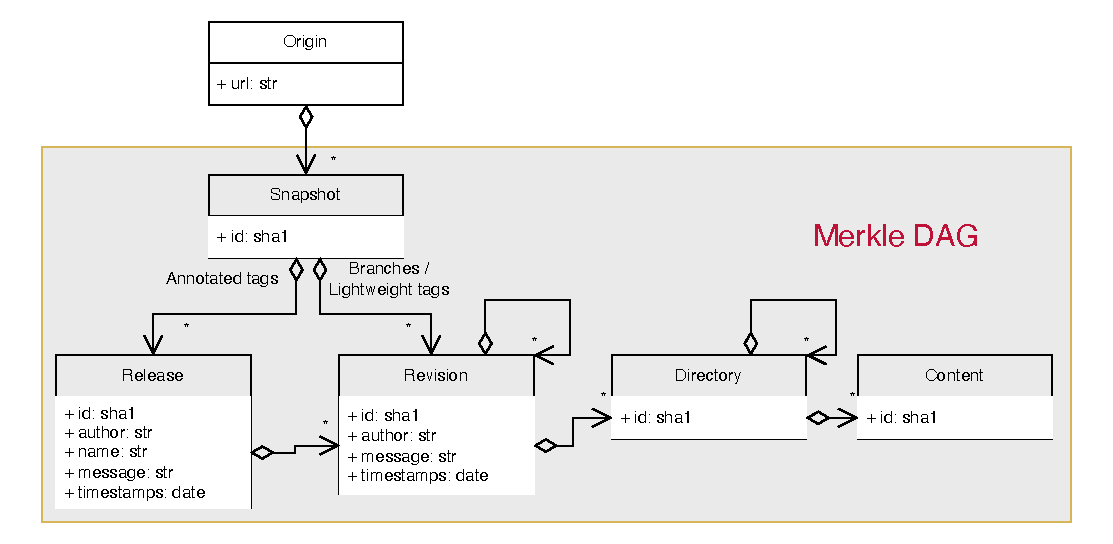
\includegraphics[width=\linewidth,height=0.66\textheight,keepaspectratio]{SWH_arch.drawio.pdf}
    \end{center}
    {\small Repeated visits yield snapshots recording the visible references --- branches and
     tags --- plus the content-addressed Merkle DAG they designate.}
\end{frame}

\begin{frame}{Backup --- snapshot-pair method}
    \hspace*{-14mm}%
    \begin{minipage}{\dimexpr\textwidth+14mm\relax}
    \centering
    \includegraphics[width=\linewidth,height=0.62\textheight,keepaspectratio]%
                    {fig_swh_snapshots.drawio.pdf}
    \end{minipage}
    {\small Two archival visits give a before/after pair; the earlier snapshot can retain
     objects the forge no longer advertises, so both sides of an alteration stay comparable.}
\end{frame}

\begin{frame}[fragile]{Backup --- Nixpkgs: from alteration to build failure}
    \begin{itemize}
        \item \NixPkgsTracked{} packages reference altered-tag origins; \NixPkgsAffected{}
              altered tags appear in recipes.
        \item \NixPkgsHashMismatch{} confirmed rebuild failures without binary cache:
              \NixPkgsFailDeletion{} deletions (availability), \NixPkgsFailHashMismatch{}
              hash mismatches (integrity).
    \end{itemize}
    \begin{lstlisting}[basicstyle=\ttfamily\footnotesize,breaklines=true,frame=single]
$ nix build ...#libv3270.src --rebuild --no-link --impure -L
error: hash mismatch in fixed-output derivation:
  specified: sha256-...
  got:       sha256-...
    \end{lstlisting}
\end{frame}

\begin{frame}{Backup --- alteration prevalence by popularity}
    \begin{center}
        \includegraphics[width=0.62\linewidth,height=0.7\textheight,keepaspectratio]%
                        {popularity_proportion.pdf}
    \end{center}
    {\small $P(\geq 1$ tag alteration$)$ rises with stars:
     \StarPropZeroOnePct{} (0--1) $\rightarrow$ \StarPropFiveHundredPlusPct{} (501+),
     even though \StarZeroOneAlterationsPercent{} of alterations sit in the 0--1 star long tail.}
\end{frame}

\begin{frame}{Backup --- secrets: refined filename patterns}
    \begin{center}
    \small
    \begin{tabular}{@{}p{3.8cm}p{7.6cm}@{}}
        \toprule
        \textbf{Group} & \textbf{Regular expression (on basename)} \\
        \midrule
        SSH key names          & \texttt{id\_rsa}, \texttt{id\_ed25519}, \texttt{id\_ecdsa}, \texttt{id\_dsa} \\
        Key containers         & \texttt{*.pem}, \texttt{*.key}, \texttt{*.pfx}, \texttt{*.p12} \\
        Environment files      & \texttt{*.env} \\
        Infra variables        & \texttt{*.tfvars} \\
        Credential-like names  & \texttt{*credentials*}, \texttt{*token*}, \texttt{*secret*}, \texttt{*config*} \\
        \bottomrule
    \end{tabular}
    \end{center}
    {\small Broad pass $\approx$ \SecretFirstExtractionShort{} records; refined pass
     $\approx$ \SecretSecondExtractionShort{} candidates (reduction $\approx 128{:}1$).}
\end{frame}

\begin{frame}[fragile]{Backup --- Tier C predefined network checks}
    \begingroup\small One read-only / metadata-only probe per family, only after written
    authorisation.\par\endgroup
    \begin{lstlisting}[basicstyle=\ttfamily\footnotesize,breaklines=true,frame=single]
# SSH private key (GitHub): active iff banner "Hi <user>!"
ssh -i ./key -o IdentitiesOnly=yes -T git@github.com

# GitHub PAT: active iff HTTP 200
curl -H "Authorization: Bearer ghp_..." https://api.github.com/user

# AWS access key: active iff account ARN returned
aws sts get-caller-identity

# OpenAI API key: active iff HTTP 200
curl -H "Authorization: Bearer sk-..." https://api.openai.com/v1/models
    \end{lstlisting}
\end{frame}

\begin{frame}{Backup --- The filename heuristic works: hit-rate by file type}
    % \begin{columns}[T,totalwidth=\textwidth]
    %     \begin{column}{0.55\textwidth}
            \centering
            % \small
            \begin{tabular}{lrr}
                \toprule
                \textbf{File type} & \textbf{Blobs} & \textbf{Rate} \\
                \midrule
                \texttt{id\_dsa}     & \num{14}    & \SI{100.0}{\percent} \\
                \texttt{id\_rsa}     & \num{129}   & \SI{81.4}{\percent}  \\
                \texttt{.key}        & \num{8270}  & \SI{57.2}{\percent}  \\
                \texttt{.pem}        & \num{26641} & \SI{24.2}{\percent}  \\
                \texttt{.env}        & \num{14705} & \SI{13.7}{\percent}  \\
                \texttt{.yml}        & \num{69586} & \SI{10.6}{\percent}  \\
                \texttt{.json}       & \num{31190} & \SI{5.8}{\percent}   \\
                \texttt{.py}         & \num{58065} & \SI{1.5}{\percent}   \\
                \texttt{.xml}        & \num{19647} & \SI{1.0}{\percent}   \\
                \bottomrule
            \end{tabular}
    %     \end{column}
    %     \begin{column}{0.42\textwidth}
    %         \begin{itemize}
    %             \item Key-material names almost always convert to a finding.
    %             \item Broad source/config extensions add \textbf{volume, little signal}.
    %             \item The refined pass concentrates the sample on names that pay off ---
    %                   and gives a \textbf{priority order} for validation.
    %         \end{itemize}
    %     \end{column}
    % \end{columns}
\end{frame}

\begin{frame}{Backup --- What kind of secrets? Private keys dominate}
    \begin{center}
    % \small
    \begin{tabular}{lr@{\hskip 1.2cm}lr}
        \toprule
        \multicolumn{2}{c}{\textbf{gitleaks}} & \multicolumn{2}{c}{\textbf{TruffleHog}} \\
        \textbf{Type} & \textbf{Count} & \textbf{Type} & \textbf{Count} \\
        \midrule
        \texttt{generic-api-key}     & \num{24133} & \texttt{PrivateKey}         & \num{19157} \\
        \texttt{private-key}         & \num{22275} & \texttt{JDBC}               & \num{6299}  \\
        \texttt{gcp-api-key}         & \num{739}   & \texttt{Circle}             & \num{1737}  \\
        \texttt{jwt}                 & \num{200}   & \texttt{MongoDB}            & \num{801}   \\
        \texttt{aws-access-token}    & \num{107}   & \texttt{Postgres}           & \num{764}   \\
        \texttt{stripe-access-token} & \num{59}    & \texttt{GoogleGeminiAPIKey} & \num{723}   \\
        \bottomrule
    \end{tabular}
    \end{center}
\end{frame}

\begin{frame}{Backup --- Tier A: are the private keys even real?}
    % \begin{center}
    % \small
    \centering
    \begin{tabular}{lrrrr}
        \toprule
        \textbf{Detector} & \textbf{Blobs} & \textbf{valid} & \textbf{encrypted} & \textbf{invalid} \\
        \midrule
        Gitleaks   & \num{11613} & \num{10038} (\SI{86.4}{\percent}) & \num{1091} (\SI{9.4}{\percent}) & \num{479} (\SI{4.1}{\percent}) \\
        TruffleHog & \num{9812}  & \num{9444} (\SI{96.3}{\percent})  & \num{134} (\SI{1.4}{\percent})  & \num{232} (\SI{2.4}{\percent}) \\
        \bottomrule
    \end{tabular}
    % \end{center}
    % \begin{itemize}
    %     \item Tier A = \textbf{offline} parsing (\texttt{ssh-keygen}, OpenSSL). No network traffic.
    %     \item \SecretPKValidBlobs{} of \SecretPKFlaggedBlobs{} gitleaks private-key blobs parse as
    %           \textbf{cryptographically valid} (\SecretPKValidPct).
    %     \item TruffleHog is the better pre-filter; gitleaks-only matches carry most scanner noise.
    %     \item \textbf{But:} syntactic validity $\neq$ active --- a revoked key still parses.
    % \end{itemize}
\end{frame}

\end{document}
